\documentclass{beamer}

\mode<presentation> {

% The Beamer class comes with a number of default slide themes
% which change the colors and layouts of slides. Below this is a list
% of all the themes, uncomment each in turn to see what they look like.

%\usetheme{default}
%\usetheme{AnnArbor}
%\usetheme{Antibes}
%\usetheme{Bergen}
%\usetheme{Berkeley}
%\usetheme{Berlin}
%\usetheme{Boadilla}
%\usetheme{CambridgeUS}
%\usetheme{Copenhagen}
%\usetheme{Darmstadt}
%\usetheme{Dresden}
%\usetheme{Frankfurt}
%\usetheme{Goettingen}
%\usetheme{Hannover}
%\usetheme{Ilmenau}
%\usetheme{JuanLesPins}
%\usetheme{Luebeck}
\usetheme{Madrid}
%\usetheme{Malmoe}
%\usetheme{Marburg}
%\usetheme{Montpellier}
%\usetheme{PaloAlto}
%\usetheme{Pittsburgh}
%\usetheme{Rochester}
%\usetheme{Singapore}
%\usetheme{Szeged}
%\usetheme{Warsaw}

% As well as themes, the Beamer class has a number of color themes
% for any slide theme. Uncomment each of these in turn to see how it
% changes the colors of your current slide theme.

%\usecolortheme{albatross}
%\usecolortheme{beaver}
%\usecolortheme{beetle}
%\usecolortheme{crane}
%\usecolortheme{dolphin}
%\usecolortheme{dove}
%\usecolortheme{fly}
%\usecolortheme{lily}
%\usecolortheme{orchid}
%\usecolortheme{rose}
%\usecolortheme{seagull}
%\usecolortheme{seahorse}
%\usecolortheme{whale}
%\usecolortheme{wolverine}

\setbeamerfont{framesource}{size=\tiny}

%\setbeamertemplate{footline} % To remove the footer line in all slides uncomment this line
%\setbeamertemplate{footline}[page number] % To replace the footer line in all slides with a simple slide count uncomment this line

\setbeamertemplate{navigation symbols}{} % To remove the navigation symbols from the bottom of all slides uncomment this line
}

\usepackage{graphicx, caption} % Allows including images
\usepackage{booktabs} % Allows the use of \toprule, \midrule and \bottomrule in tables
\usepackage[absolute,overlay]{textpos}
\usepackage{epstopdf} %converting to PDF
\usepackage{amssymb}
\usepackage{amsmath}

\newcommand{\source}[1]{\begin{textblock*}{4cm}(8.7cm,8.6cm)
    \begin{beamercolorbox}[ht=0.5cm,right]{framesource}
        \usebeamerfont{framesource}\usebeamercolor[fg]{framesource} Source: {#1}
    \end{beamercolorbox}
\end{textblock*}}

\newcommand{\image}[1]{\begin{textblock*}{4cm}(8.7cm,8.6cm)
    \begin{beamercolorbox}[ht=0.5cm,right]{framesource}
        \usebeamerfont{framesource}\usebeamercolor[fg]{framesource} Image: {#1}
    \end{beamercolorbox}
\end{textblock*}}

%----------------------------------------------------------------------------------------
%	TITLE PAGE
%----------------------------------------------------------------------------------------

\title[Haplotype-based somatic mutation calling]{Haplotype-based somatic mutation calling in heterogeneous cancer samples”} % The short title appears at the bottom of every slide, the full title is only on the title page

\author[Daniel Cooke]{Daniel Cooke}

\institute[Oxford University] % Your institution as it will appear on the bottom of every slide, may be shorthand to save space
{
University of Oxford \\ % Your institution for the title page
\medskip
\textit{dcooke@well.ox.ac.uk} % Your email address
}
\date{\today} % Date, can be changed to a custom date

\begin{document}

\begin{frame}
\titlepage % Print the title page as the first slide
\end{frame}

%----------------------------------------------------------------------------------------
%	PRESENTATION SLIDES
%----------------------------------------------------------------------------------------

%------------------------------------------------
\section{Background}
%------------------------------------------------

\begin{frame}
\frametitle{Haplotype-based variant calling}

\begin{center}
    
\includegraphics[width=0.3\linewidth]{images/gatk-logo}
    \hfill
    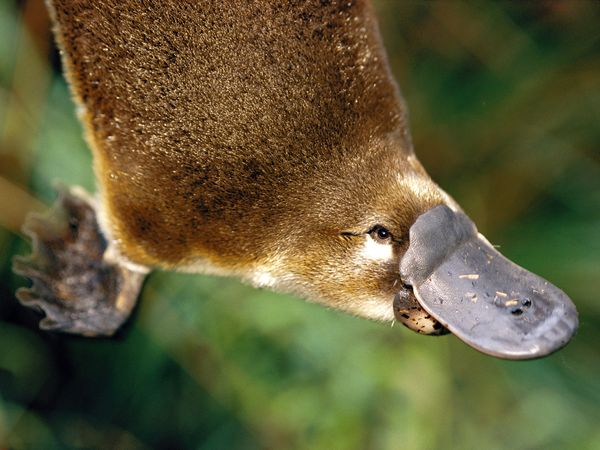
\includegraphics[width=0.3\linewidth]{images/platypus}
    \hfill
    
\includegraphics[width=0.3\linewidth]{images/freebayes}
\end{center}

\end{frame}

\begin{frame}
\frametitle{Haplotype methods can resolve alignment errors}

\begin{center}
    % Strong positional support for multiple variants but reads have same bases
    
    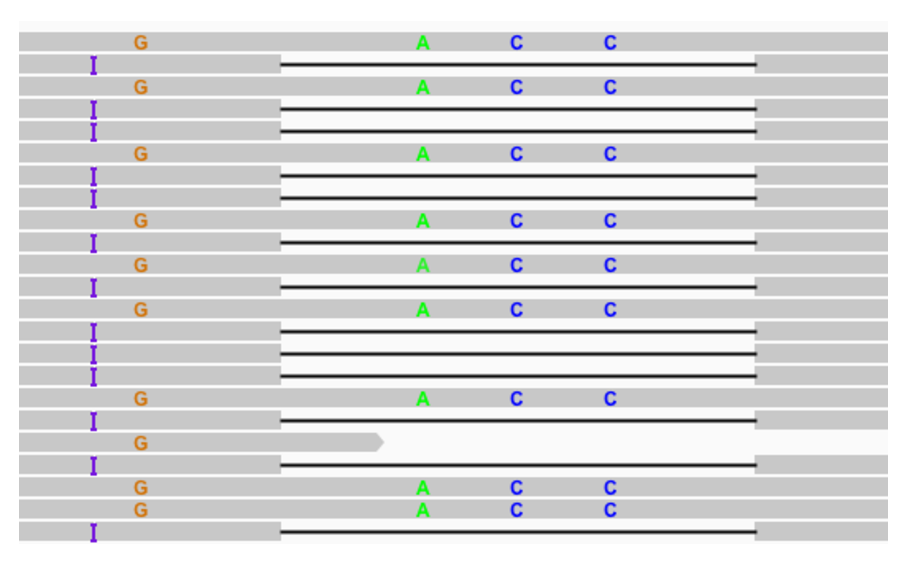
\includegraphics[height=0.7\textheight]{images/haplotype_callers1}
    
    % Haplotype methods call single complex substitution
\end{center}

\end{frame}

\begin{frame}
\frametitle{Haplotype methods can resolve alignment errors}

\begin{center}
    % Weak positional support for validated insertion due to misalignment
    
    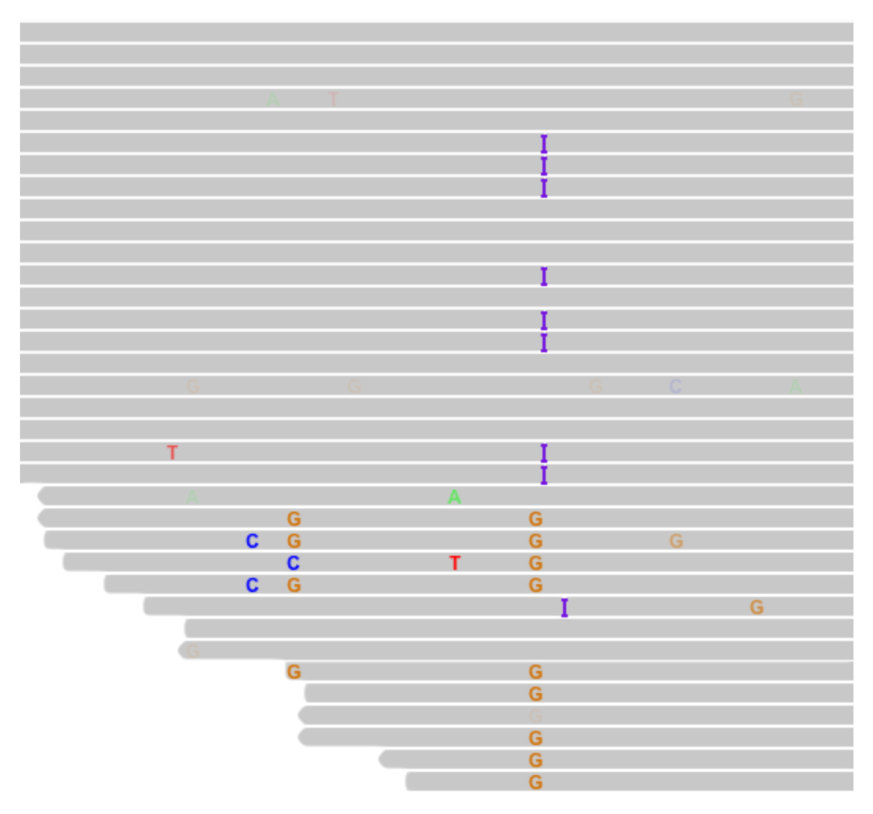
\includegraphics[height=0.8\textheight]{images/haplotype_callers2}
    
    % Haplotype methods use misaligned reads to call insertion
\end{center}

\end{frame}

%------------------------------------------------

\begin{frame}
\frametitle{Haplotype methods give local phasing}

\begin{center}
    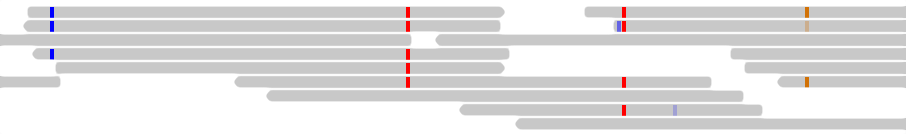
\includegraphics[width=\linewidth]{images/phasing}
\end{center}

\onslide<2->{
\centerline{First haplotype}
\begin{center}
    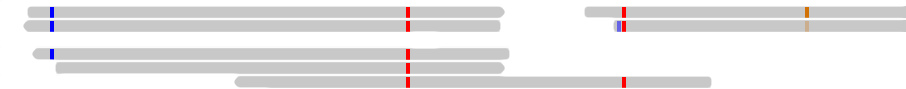
\includegraphics[width=\linewidth]{images/phased_haplotype1}
\end{center}
}

\onslide<3->{
\centerline{Second haplotype}
\begin{center}
    
\includegraphics[width=\linewidth]{images/phased_haplotype2}
\end{center}
}

\end{frame}

%------------------------------------------------
\section{Our algorithm}
%------------------------------------------------

\begin{frame}
\frametitle{Phasing is often intractable}

\begin{align*}
\#\text{haplotypes} &\approx 2^{\text{\#alleles}} \\
\#\text{genotypes} &= \binom{\#\text{haplotypes} + \text{ploidy} - 1}{\#\text{haplotypes}}
\end{align*}

\begin{exampleblock}{Example: HLA loci}

\begin{center}
    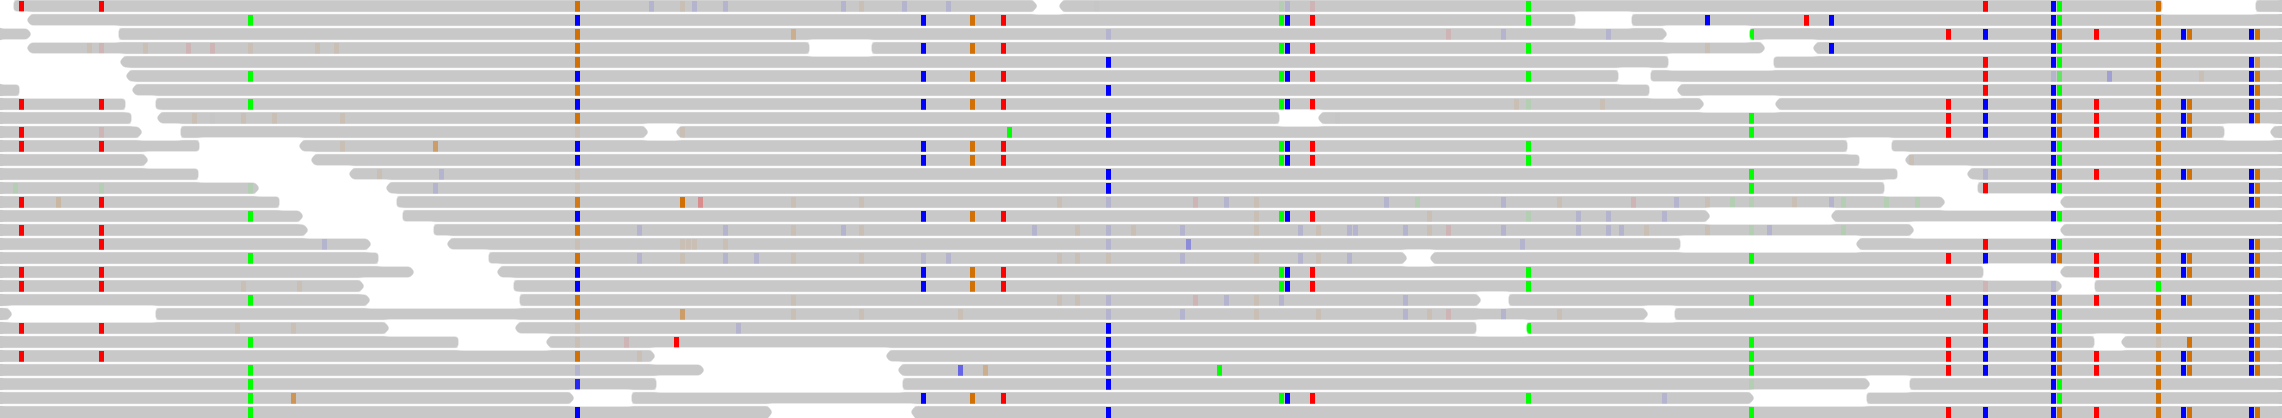
\includegraphics[width=\linewidth]{images/hla_phasing_clear}
\end{center}

\centerline{$\#\text{alleles} \approx 70 \rightarrow \#\text{haplotypes} \approx 2^{70} \rightarrow \#\text{genotypes} \approx \text{lots}$}

\end{exampleblock}

\end{frame}

%------------------------------------------------

\begin{frame}
\frametitle{Haplotype tree phasing}

\only<1>{
\begin{center}
    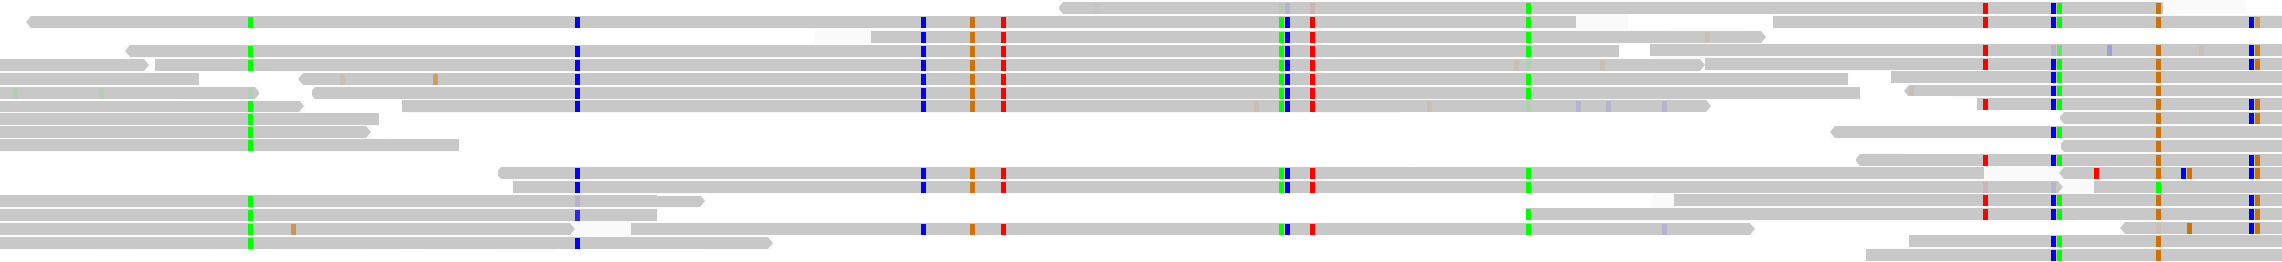
\includegraphics[width=\linewidth]{images/hla_phasing1.png}
\end{center}
\begin{center}
    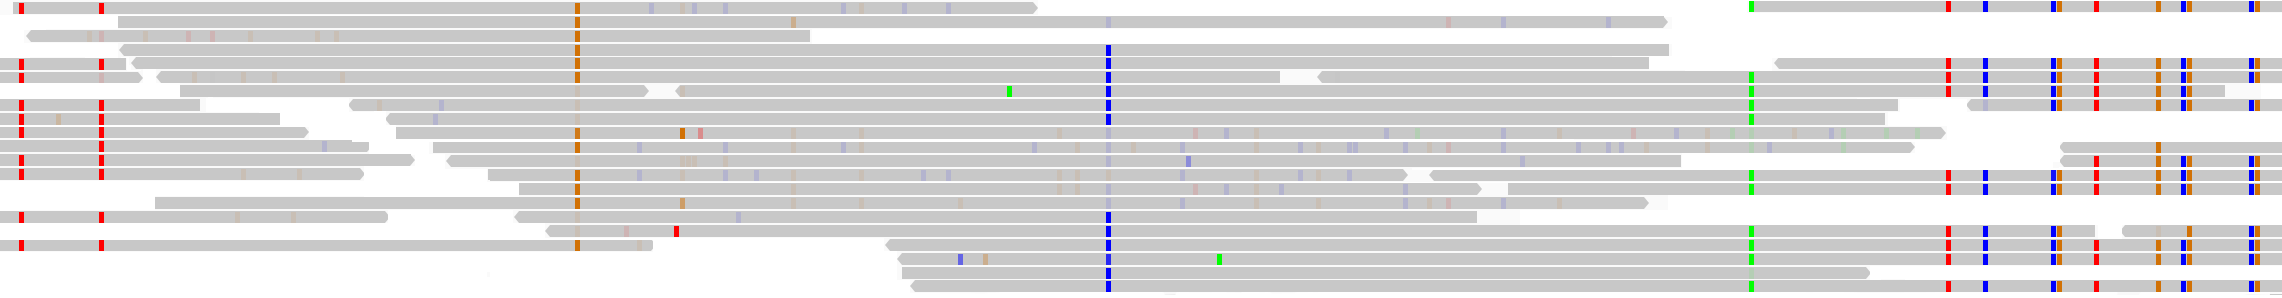
\includegraphics[width=\linewidth]{images/hla_phasing2.png}
\end{center}
}

\only<2>{
\begin{center}
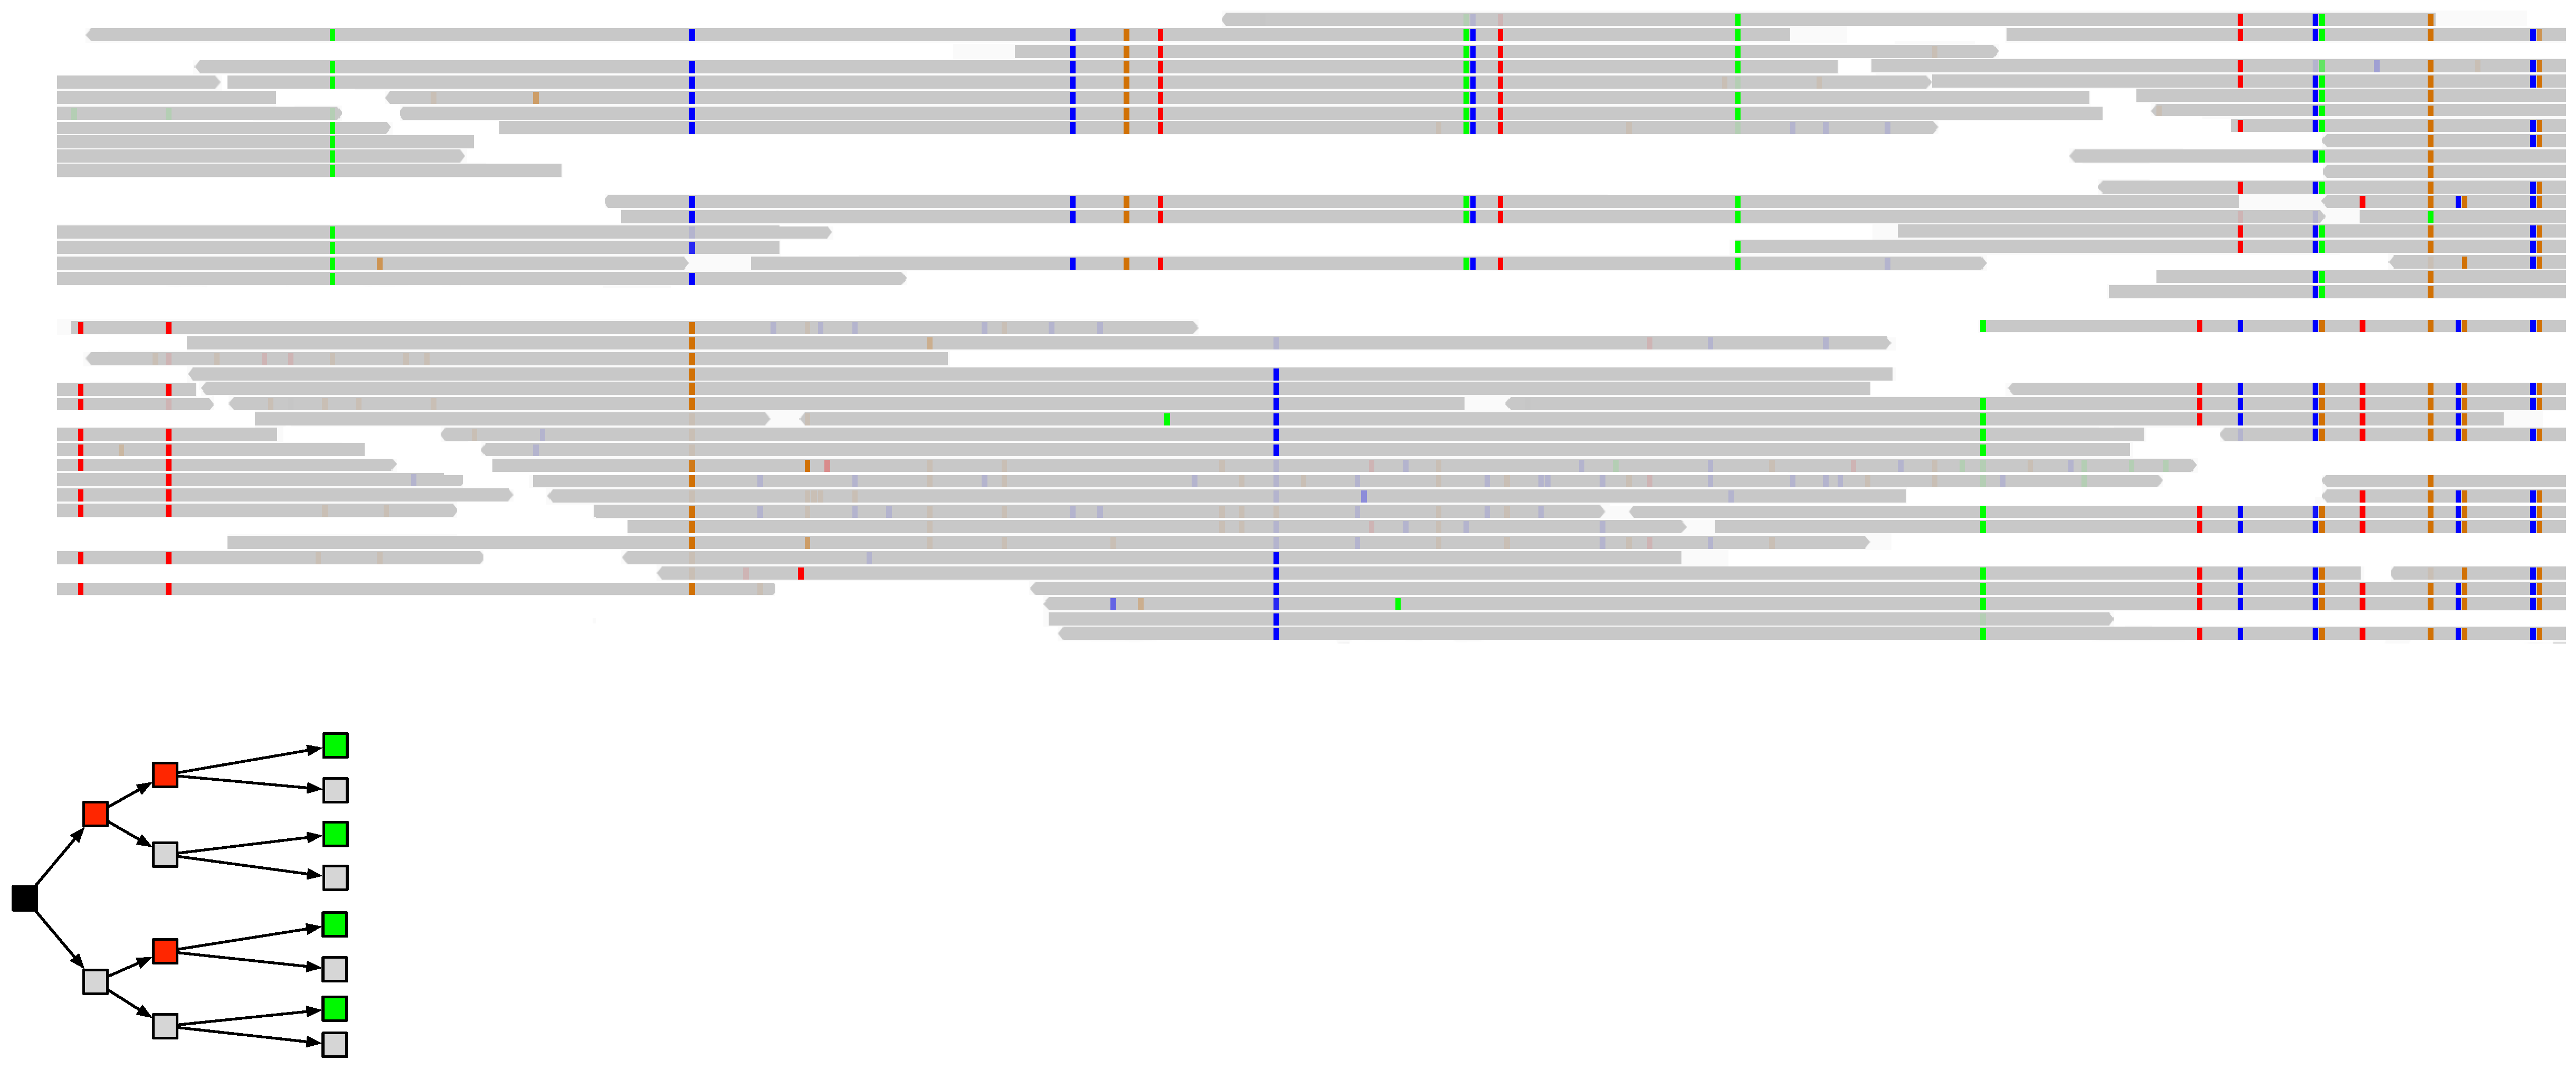
\includegraphics[width=\linewidth]{images/hla_tree1}
\end{center}
}

% \only<2>{
% Extend by a tractable number of alleles
% }

\only<3>{
\begin{center}
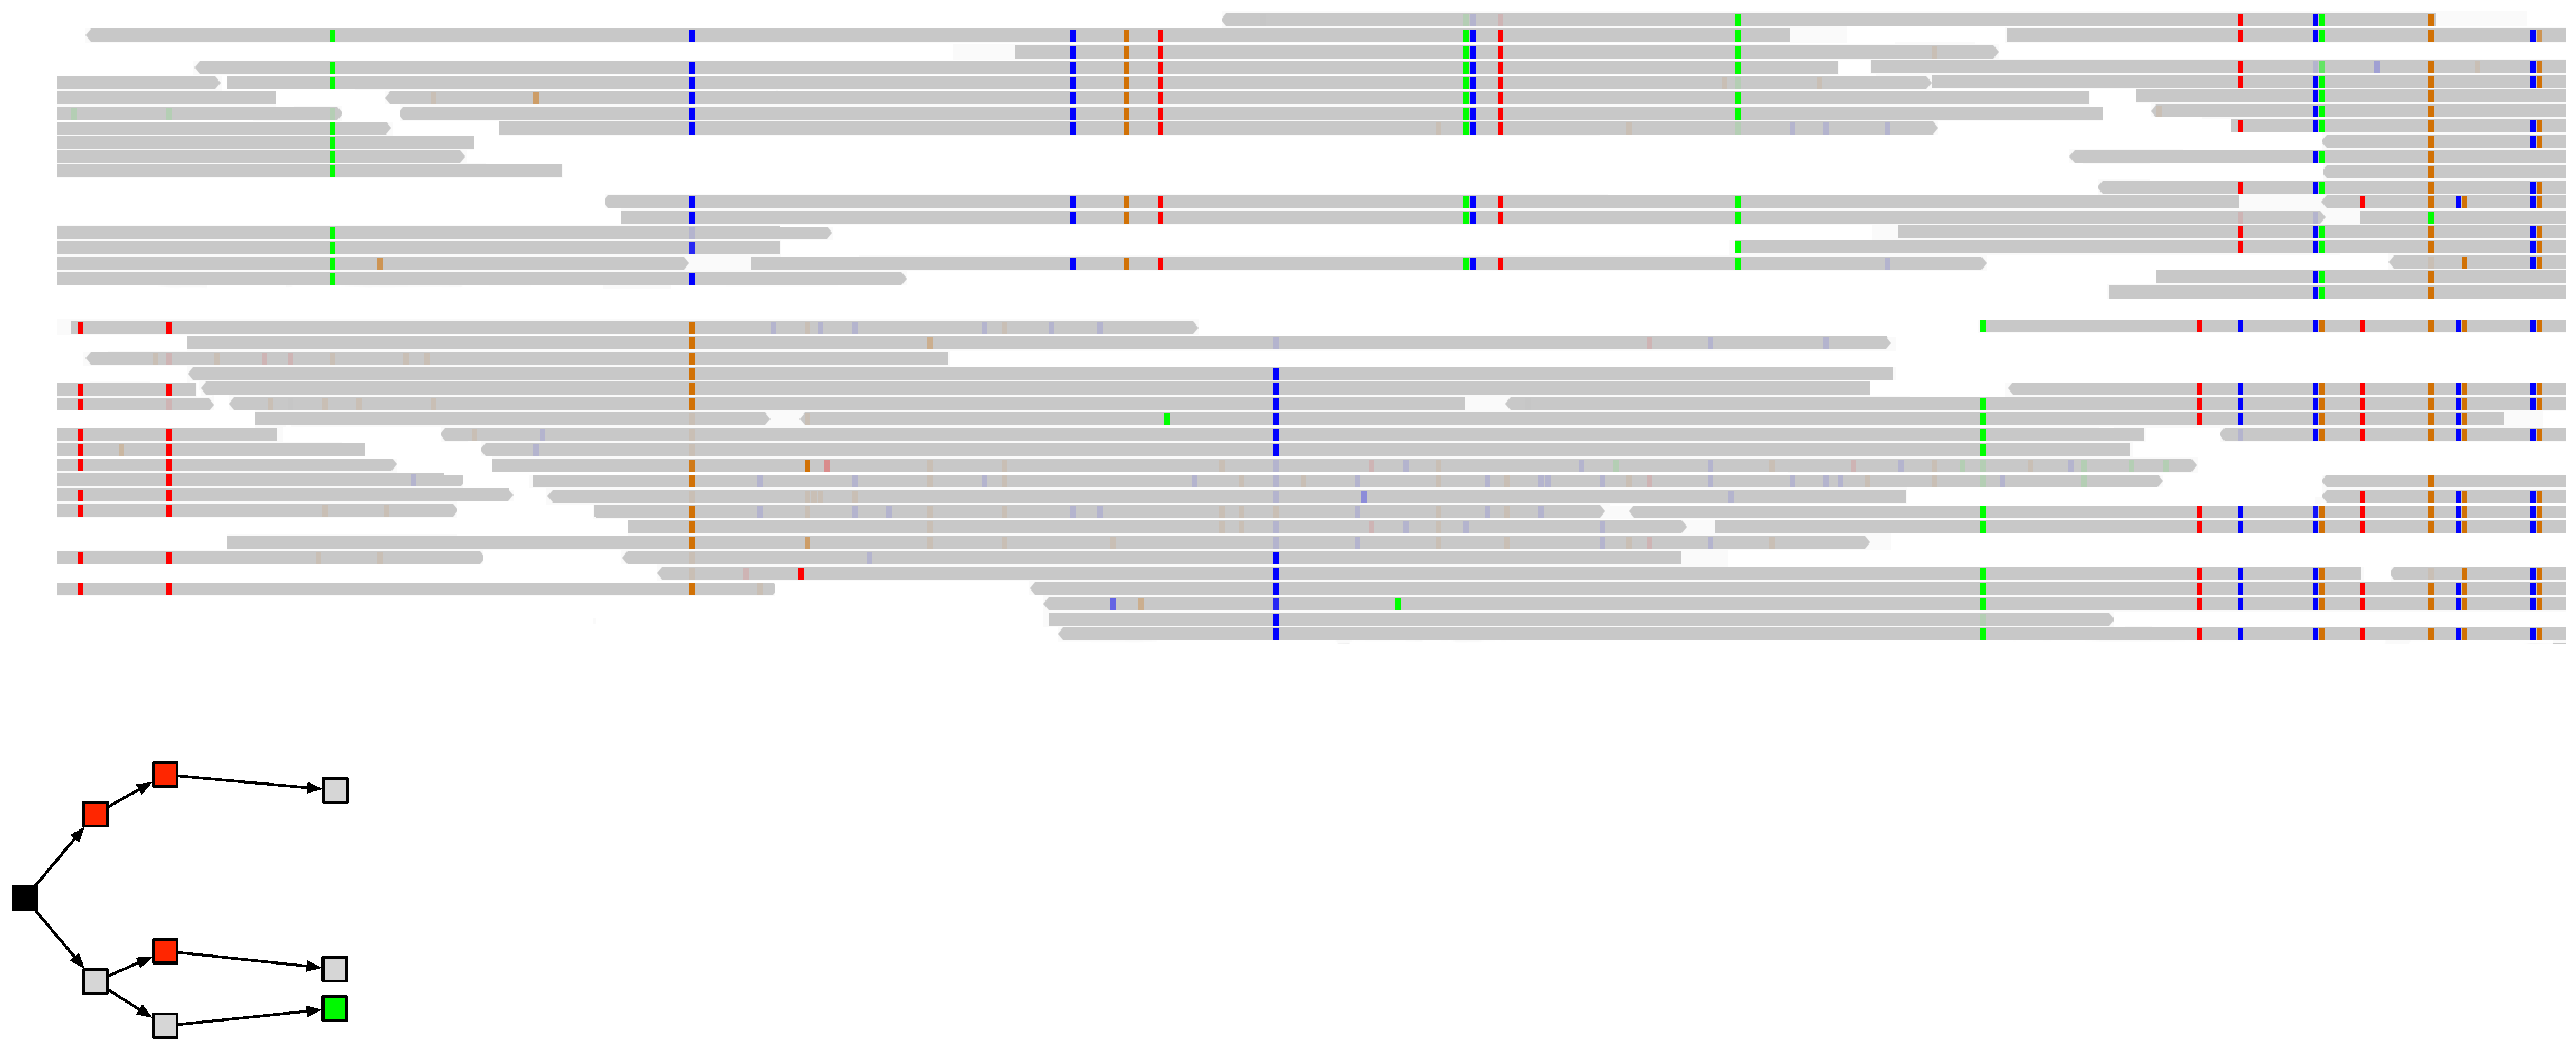
\includegraphics[width=\linewidth]{images/hla_tree2}
\end{center}
}

% \only<3>{
% Prune haplotypes with low posterior support
% }

\only<4>{
\begin{center}
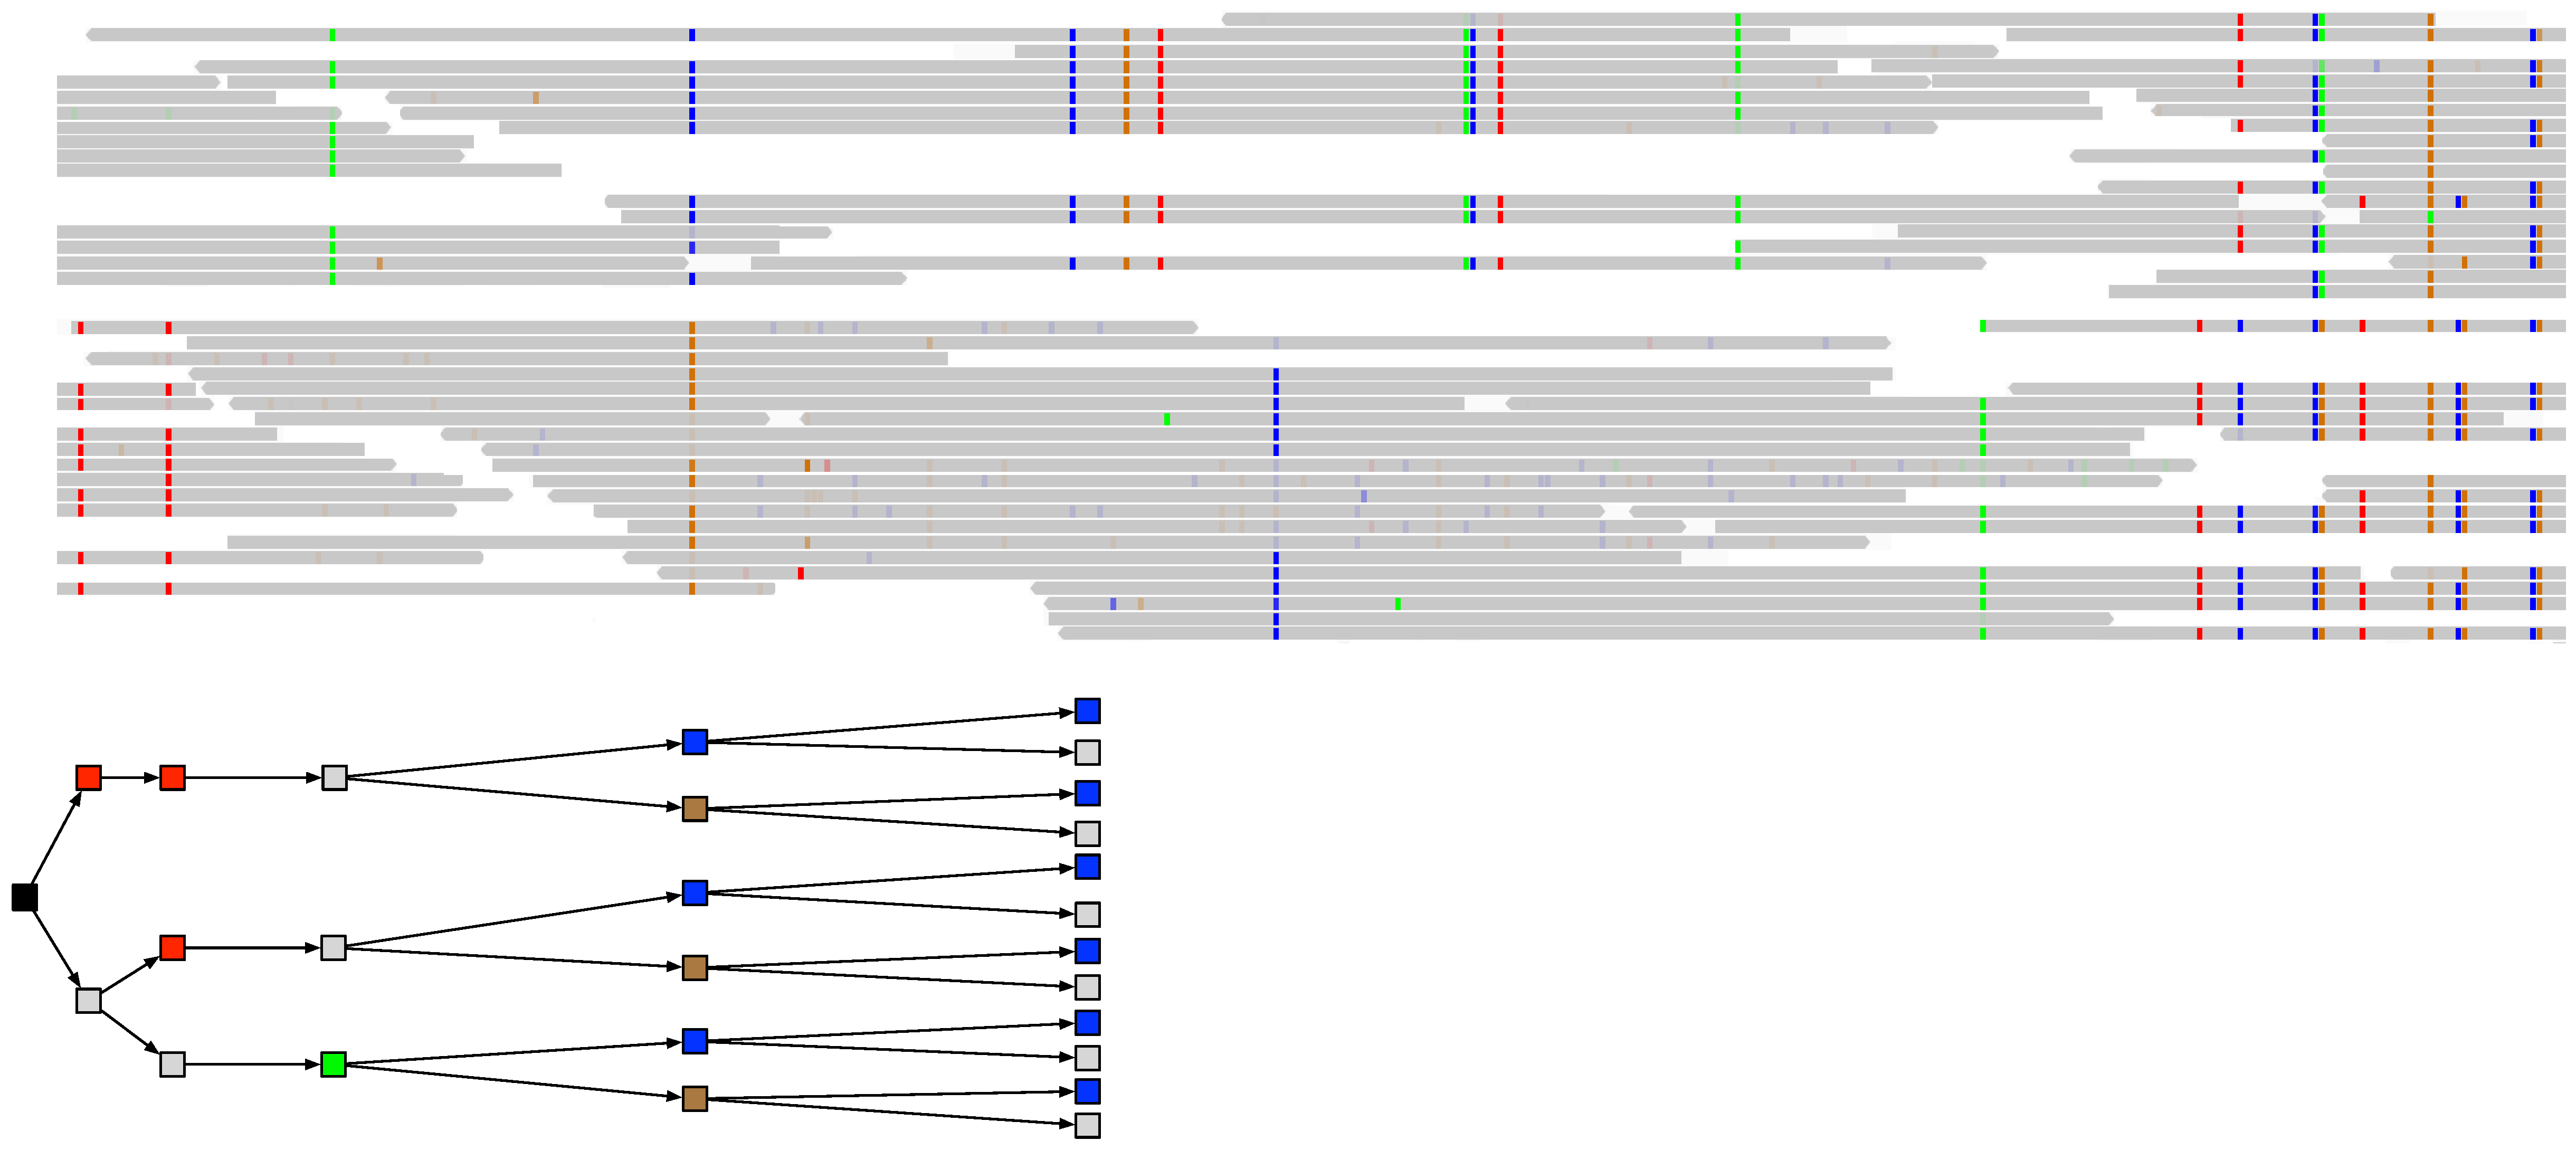
\includegraphics[width=\linewidth]{images/hla_tree3}
\end{center}
}

% \only<4>{
% Extend the pruned tree
% }

\only<5>{
\begin{center}
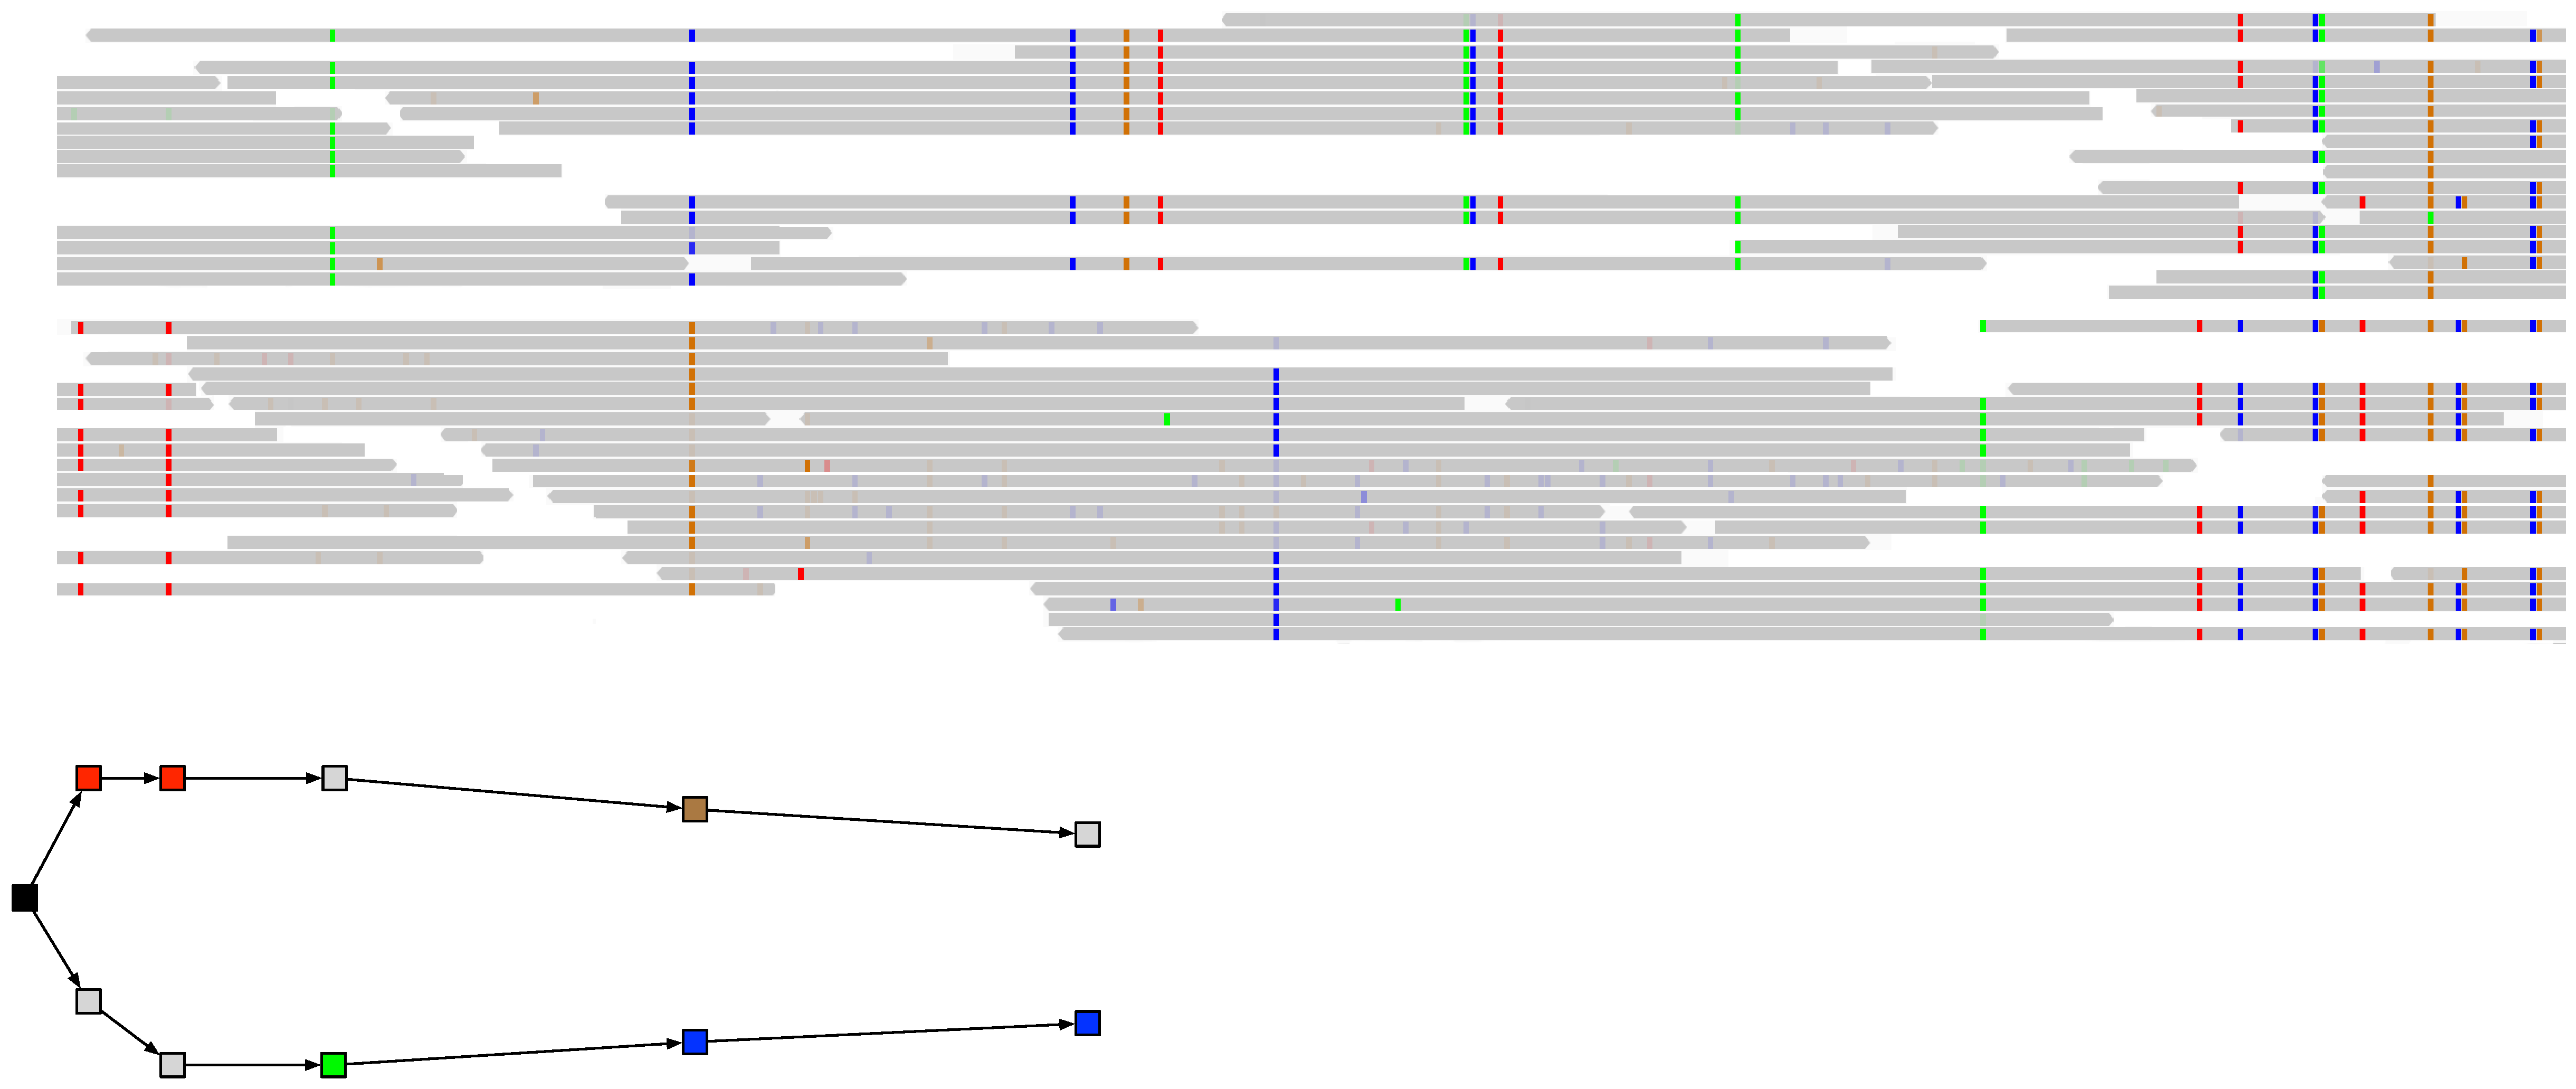
\includegraphics[width=\linewidth]{images/hla_tree4}
\end{center}
}

% \only<5>{
% Repeat until ambigous phasing or no more candidate alleles
% }

\only<6>{
\begin{center}
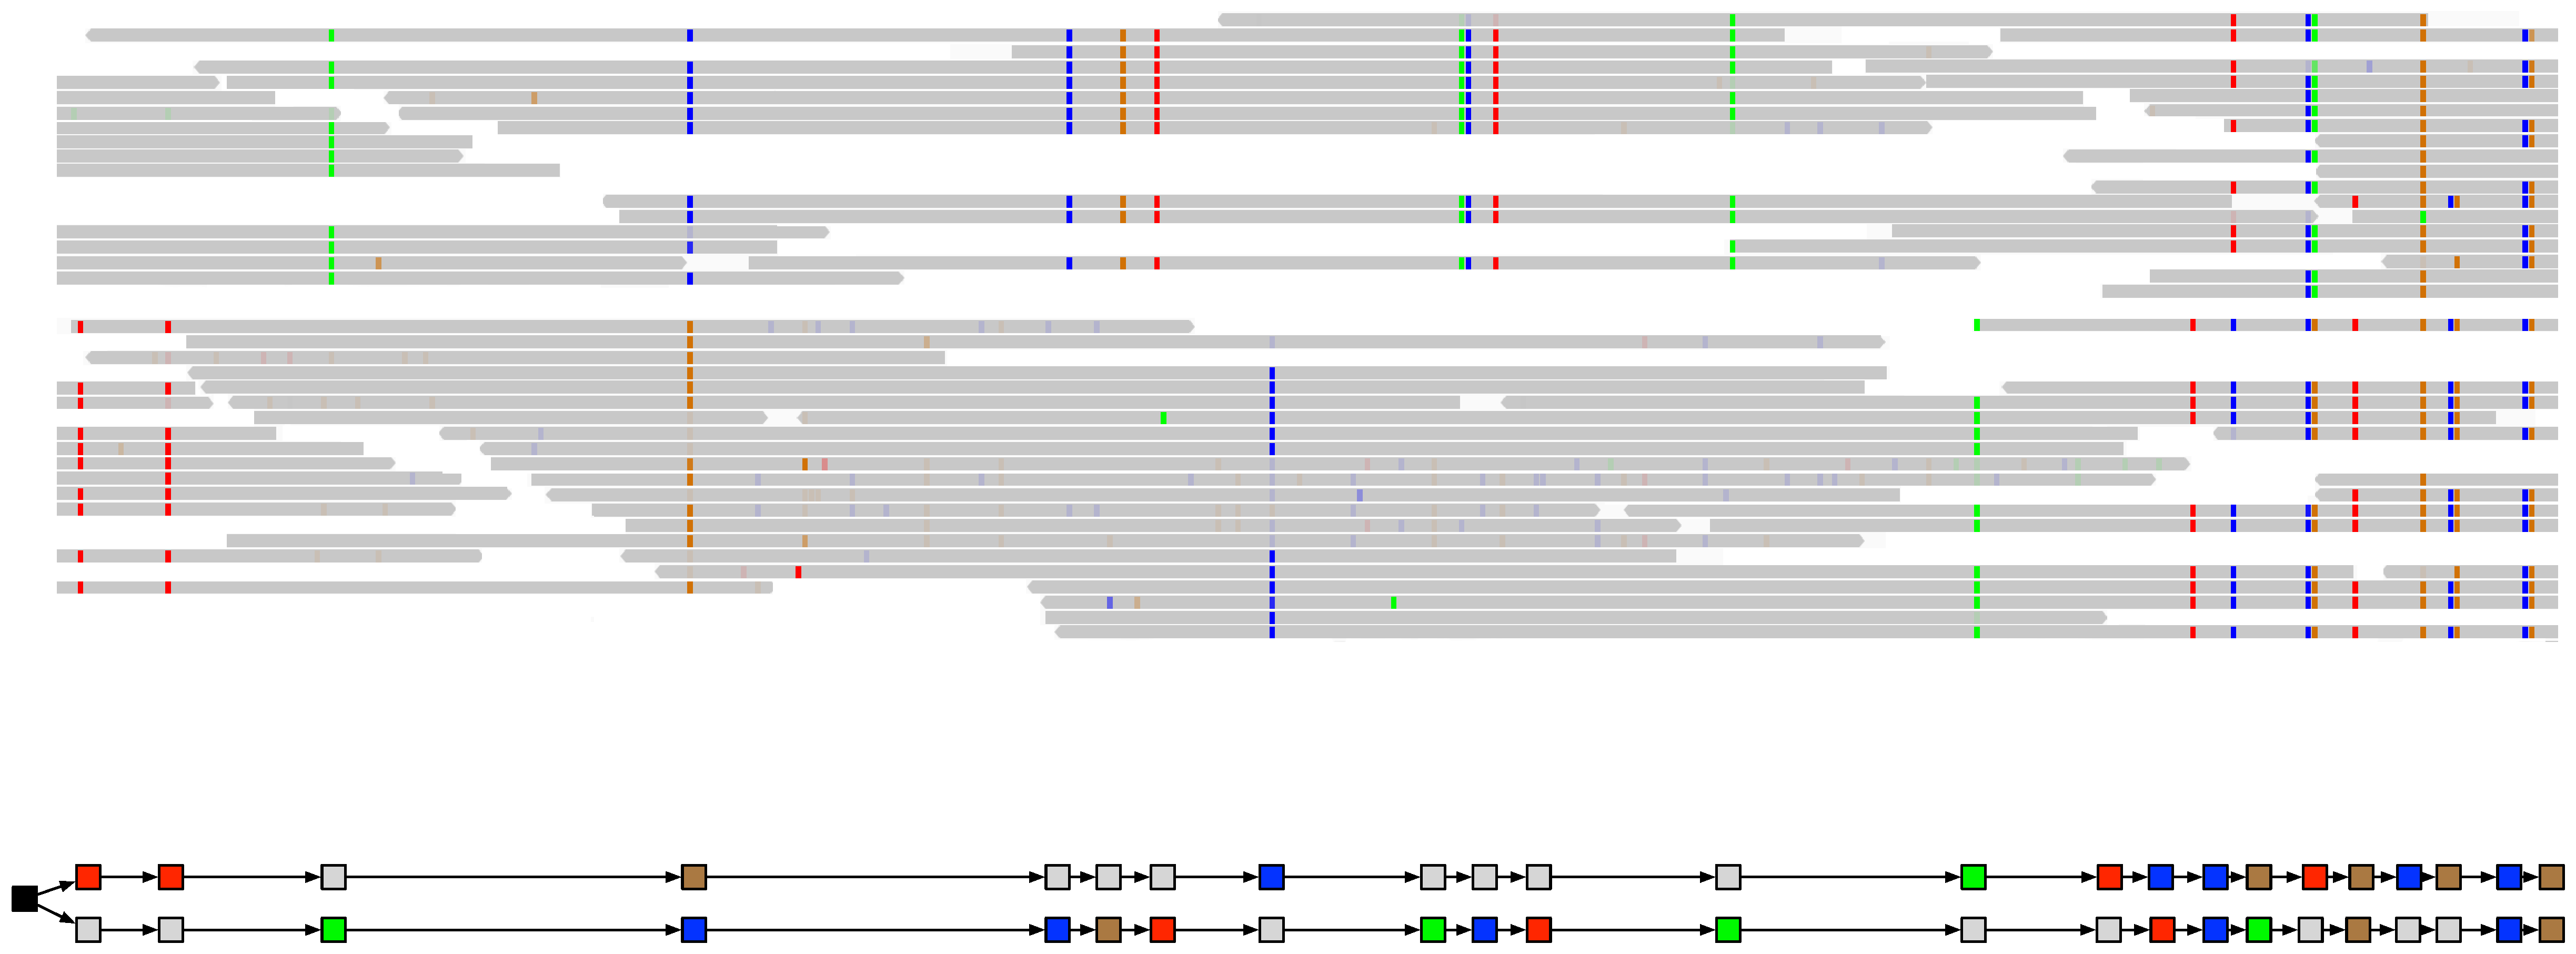
\includegraphics[width=\linewidth]{images/hla_tree5}
\end{center}
}

% \only<6>{
% Probablistic local phasing in linear time
% }

\end{frame}

%------------------------------------------------

\begin{frame}
\frametitle{Algorithm overview}
\begin{center}
    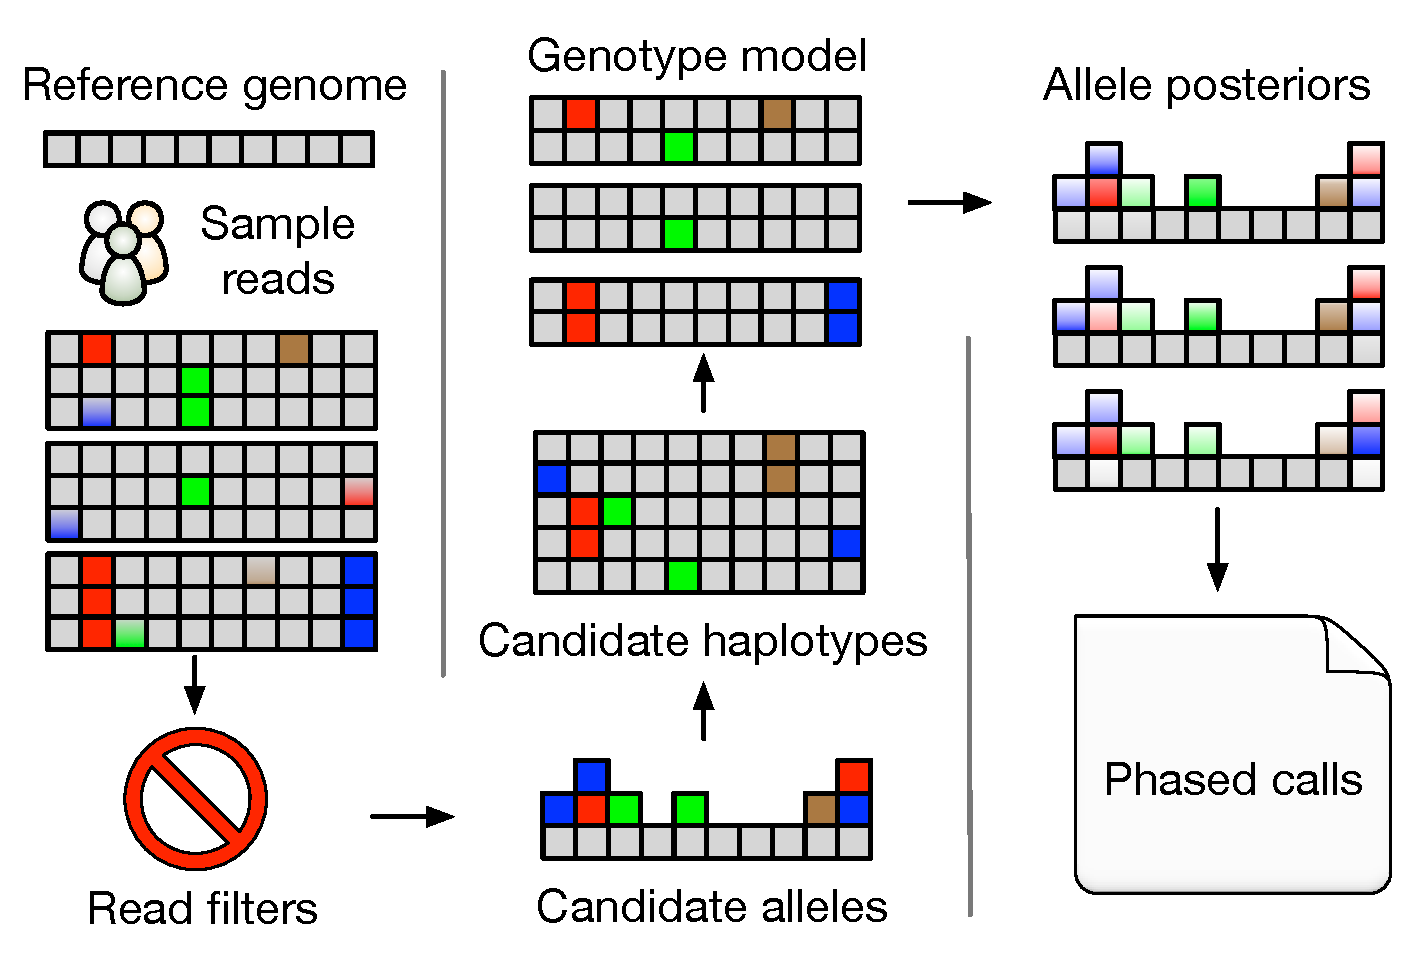
\includegraphics[width=0.95\linewidth]{images/octopus_workflow}
\end{center}
\end{frame}

%------------------------------------------------

\begin{frame}
\frametitle{Population genotype model: overview}

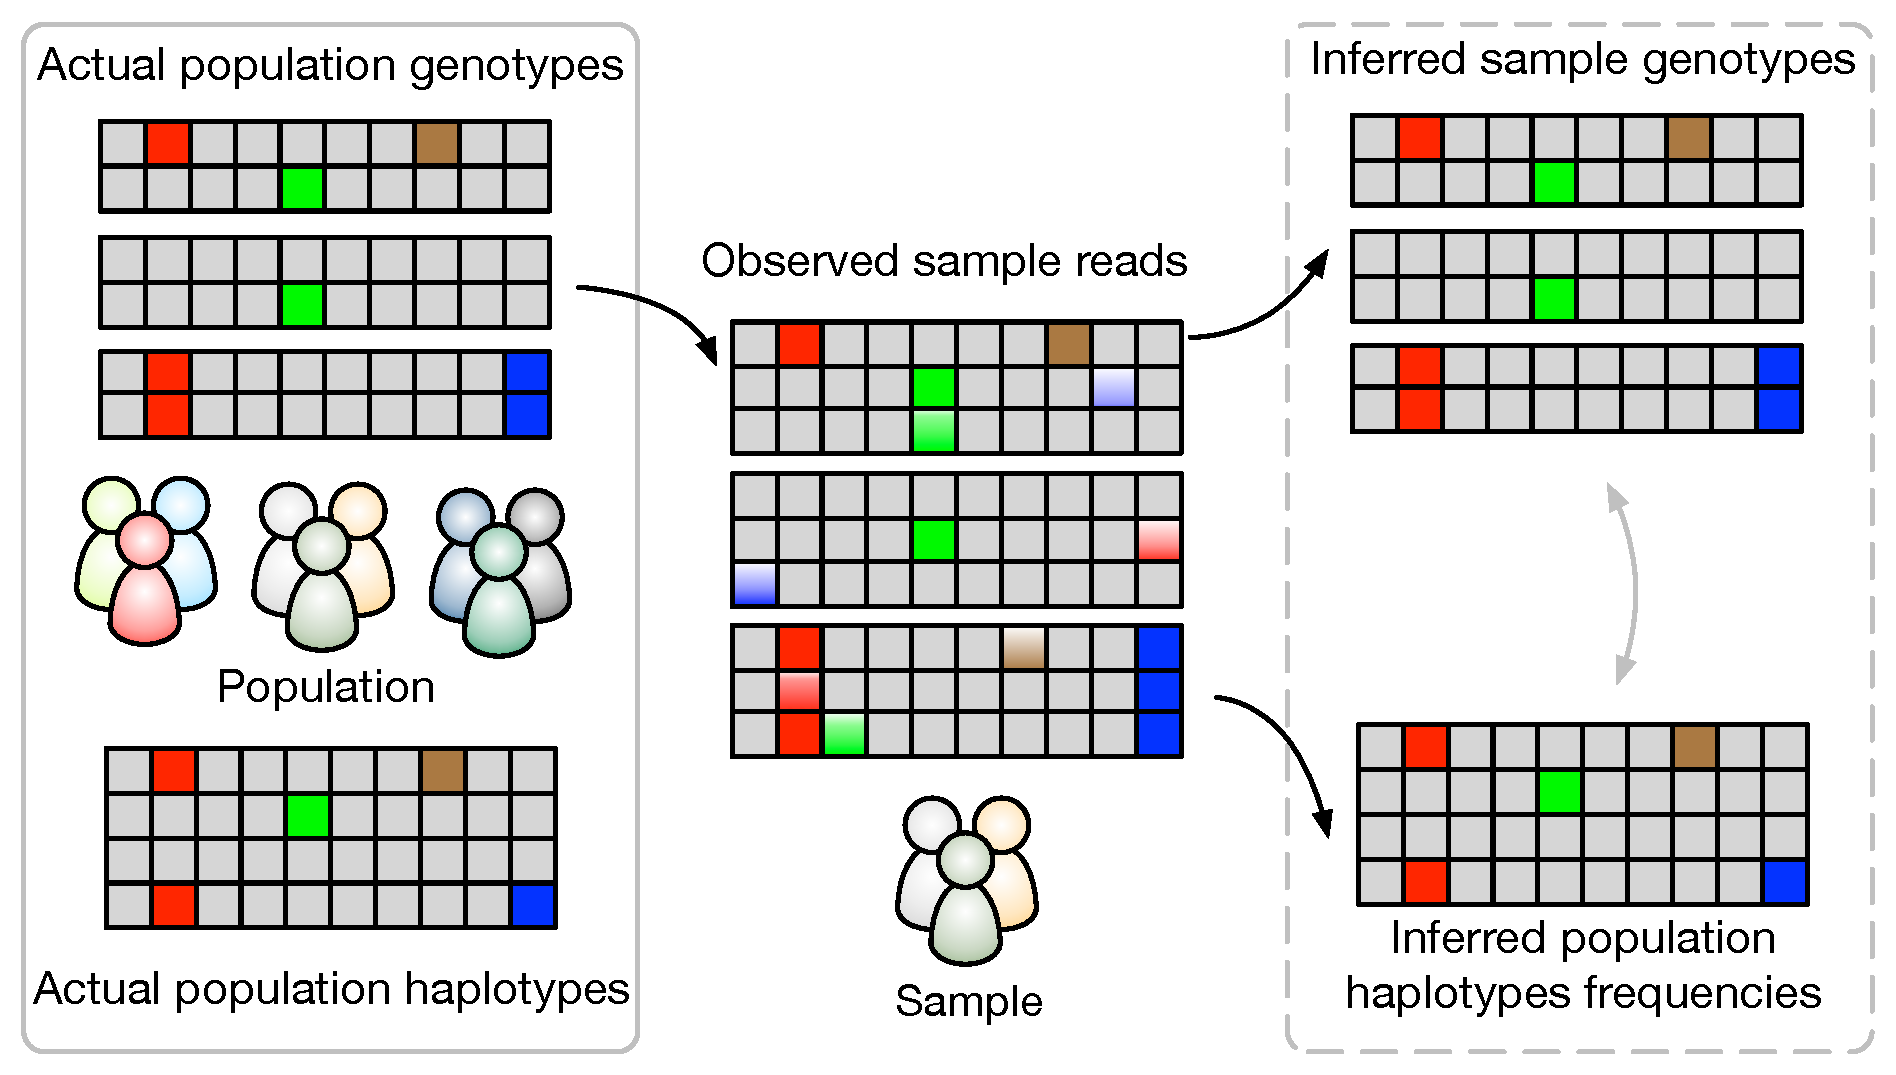
\includegraphics[width=\linewidth]{images/population_calling}

\end{frame}

%------------------------------------------------

\begin{frame}
\frametitle{Population genotype model: maths}

\begin{columns}[c]

\begin{column}{.4\textwidth}
    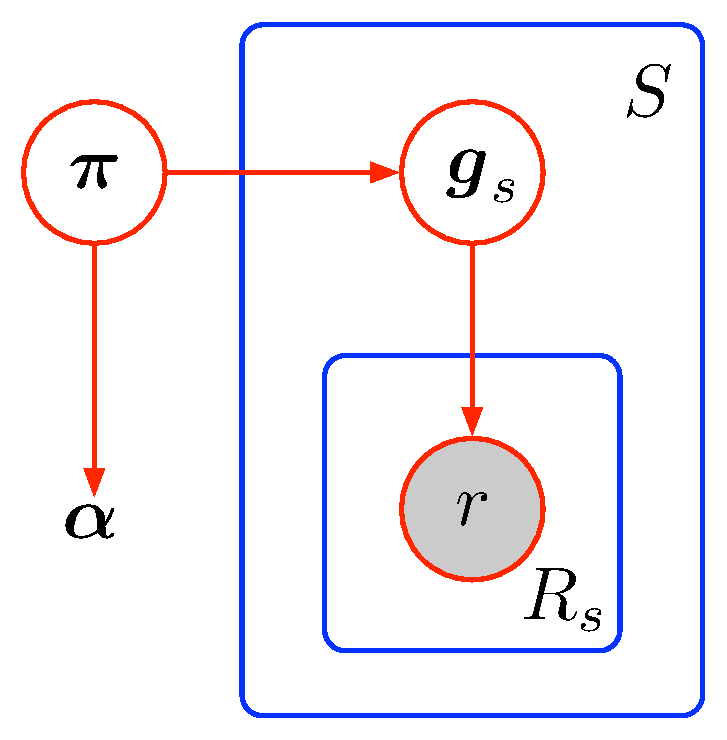
\includegraphics[width=\linewidth]{images/population_model}
\end{column}

\begin{column}{.6\textwidth}

\begin{itemize}
\item Unknown population haplotype frequencies $\boldsymbol{\pi}$
\item Unknown sample genotypes $\boldsymbol{g}_s$
\item Known sample ploidy
\end{itemize}

\end{column}
\end{columns}

\only<1>{
\begin{exampleblock}{Marginal distribution: diploid case}
\begin{equation*}
p(\boldsymbol{R}, \boldsymbol{\pi}) = p(\boldsymbol{\pi} | \boldsymbol{\alpha}) \prod_{s=1}^S \sum_{\boldsymbol{g}}  p(\boldsymbol{g} | \boldsymbol{\pi}) \prod_{r \in R_s} \left\{ \frac{1}{2} p(r | \boldsymbol{g}_1) + \frac{1}{2} p(r | \boldsymbol{g}_2) \right\}
\end{equation*}
\end{exampleblock}
}

% \only<2>{
% \begin{exampleblock}{Marginal distribution: general case}
% \begin{equation*}
% p(\boldsymbol{R}, \boldsymbol{\pi}) = p(\boldsymbol{\pi} | \boldsymbol{\alpha}) \prod_{s=1}^S \sum_{\boldsymbol{g}}  p(\boldsymbol{g} | \boldsymbol{\pi}) \prod_{r \in R_s} \frac{1}{|\boldsymbol{g}|} \sum_{i = 1}^{|\boldsymbol{g}|} p(r | \boldsymbol{g}_i)
% \end{equation*}
% \end{exampleblock}
% }

% MAP estimates of $\boldsymbol{\pi}$ and $\boldsymbol{g}_s$ using EM

\end{frame}

%------------------------------------------------

\begin{frame}
\frametitle{Challenges of cancer calling: messy karyotypes}

\begin{center}
    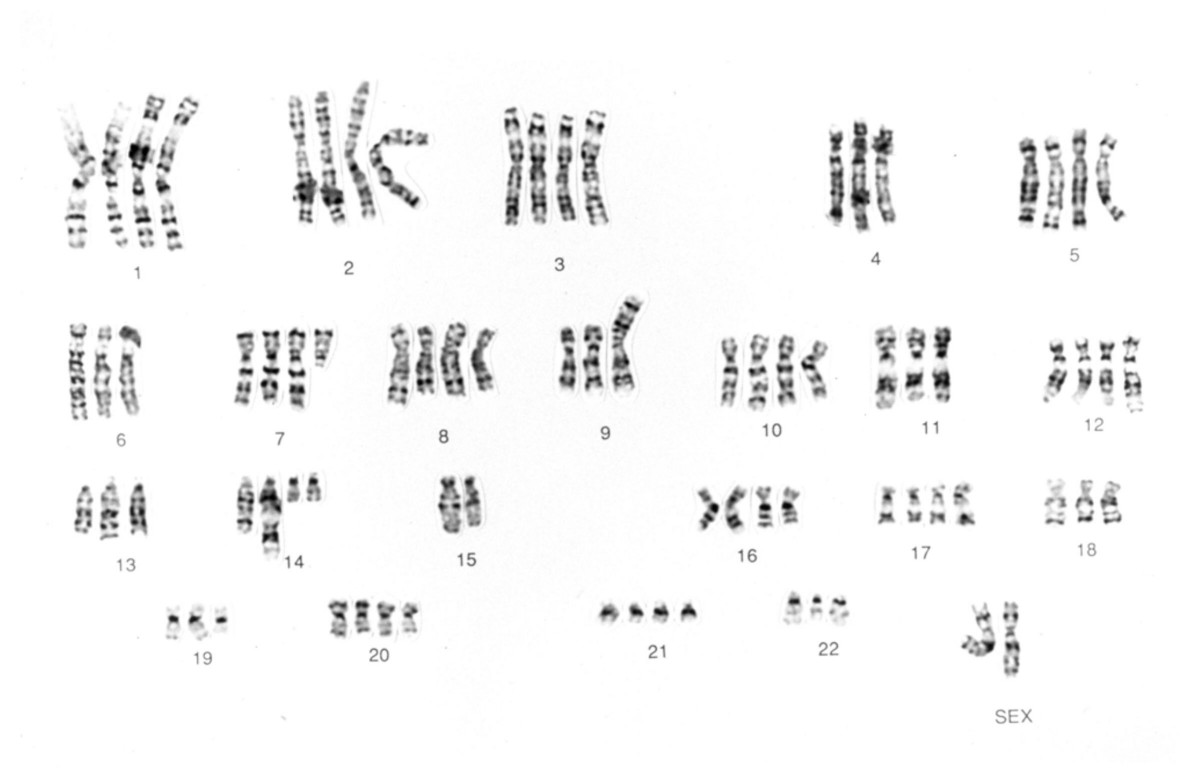
\includegraphics[width=\linewidth]{images/cancer_karyotype}
\end{center}
\source{Hillman et al. BMC Cancer 2007}

\end{frame}

%------------------------------------------------

\begin{frame}
\frametitle{Challenges of cancer calling: tumor heterogeneity}

\begin{center}
    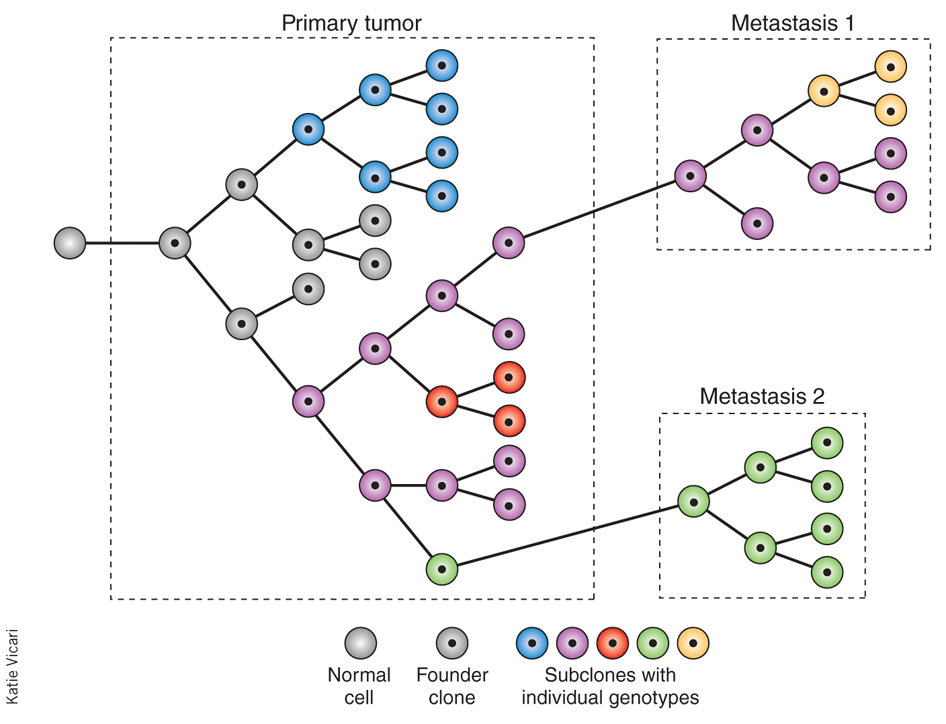
\includegraphics[width=0.85\linewidth]{images/nbt2213-F1}
\end{center}
\source{Carlos Caldas Nature Biotechnology 2012}

\end{frame}

%------------------------------------------------

\begin{frame}
\frametitle{How many haplotypes do we need?}

\begin{center}
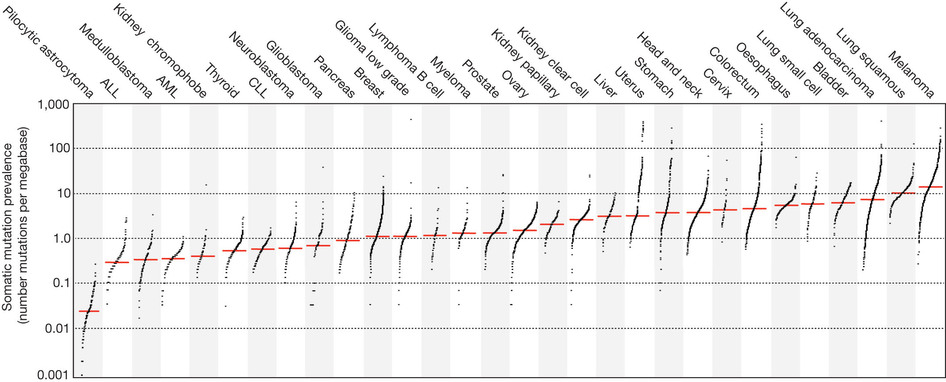
\includegraphics[width=\linewidth]{images/cancer_somatic_rates.jpg}
\end{center}
\source{Alexandrov et al. Nature 2013}

\centerline{\textbf{More than three local haplotypes are rare in most cancer types}}

\end{frame}

%------------------------------------------------

\begin{frame}
\frametitle{Cancer genotype model: overview}

\begin{center}
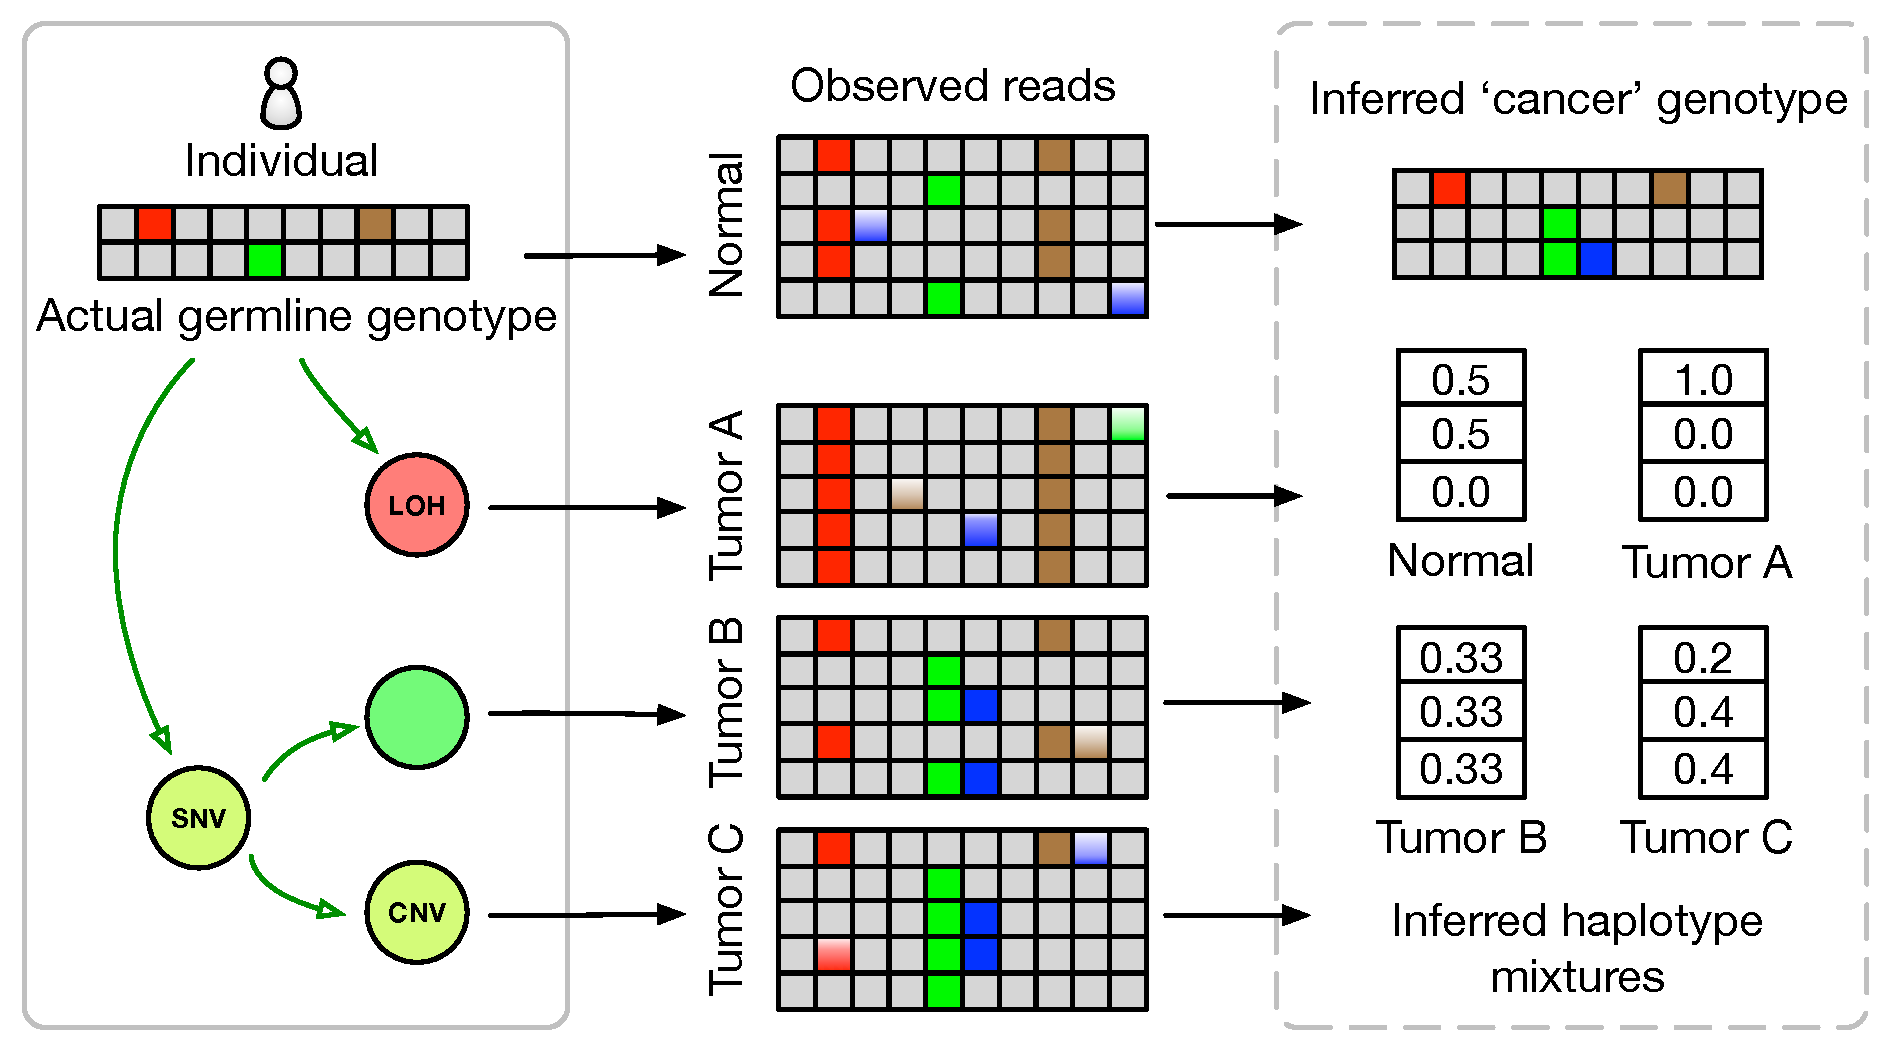
\includegraphics[width=\linewidth]{images/cancer_calling}
\end{center}

\end{frame}

%------------------------------------------------

\begin{frame}[fragile] % Need to use the fragile option when verbatim is used in the slide
\frametitle{Cancer genotype model: maths}

\begin{columns}[c]

\begin{column}{.35\textwidth}
    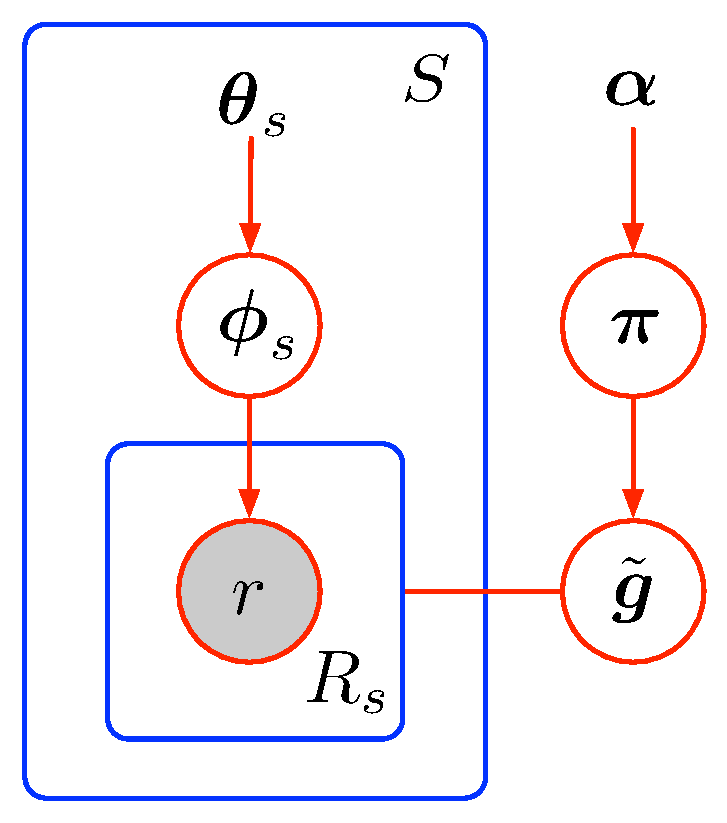
\includegraphics[width=\linewidth]{images/cancer_model}
\end{column}

\begin{column}{.65\textwidth}
\begin{itemize}
\item One unknown 'cancer' genotype $\tilde{\boldsymbol{g}}$
\item Unknown haplotype mixtures $\boldsymbol{\phi}_s$
\item Mixture priors $\boldsymbol{\theta}_s$ implicitly model 'normal'
\end{itemize}
\end{column}
\end{columns}

\begin{exampleblock}{Marginal distribution: diploid case}
\setlength\abovedisplayskip{0pt}
\begin{equation*}
p(\boldsymbol{R}, \boldsymbol{\pi}) = p(\boldsymbol{\pi} | \boldsymbol{\alpha}) \sum_{\tilde{\boldsymbol{g}}} p(\tilde{\boldsymbol{g}} | \boldsymbol{\pi}) \prod_{s=1}^S \int d \boldsymbol{\phi}_s   p(\boldsymbol{\phi}_s | \boldsymbol{\theta}_s) \prod_{r \in R_s} \sum_{i = 1}^3 p(\tilde{\boldsymbol{g}}_i | \boldsymbol{\phi}_{si}) p(r | \tilde{\boldsymbol{g}}_i)
\end{equation*}
\end{exampleblock}

% MAP estimates of $\boldsymbol{\phi}_s$ and $\tilde{\boldsymbol{g}}$ using EM

\end{frame}

%------------------------------------------------
\section{Results}
%------------------------------------------------

\begin{frame}
\frametitle{Phased somatic mutation calls}

\begin{center}
    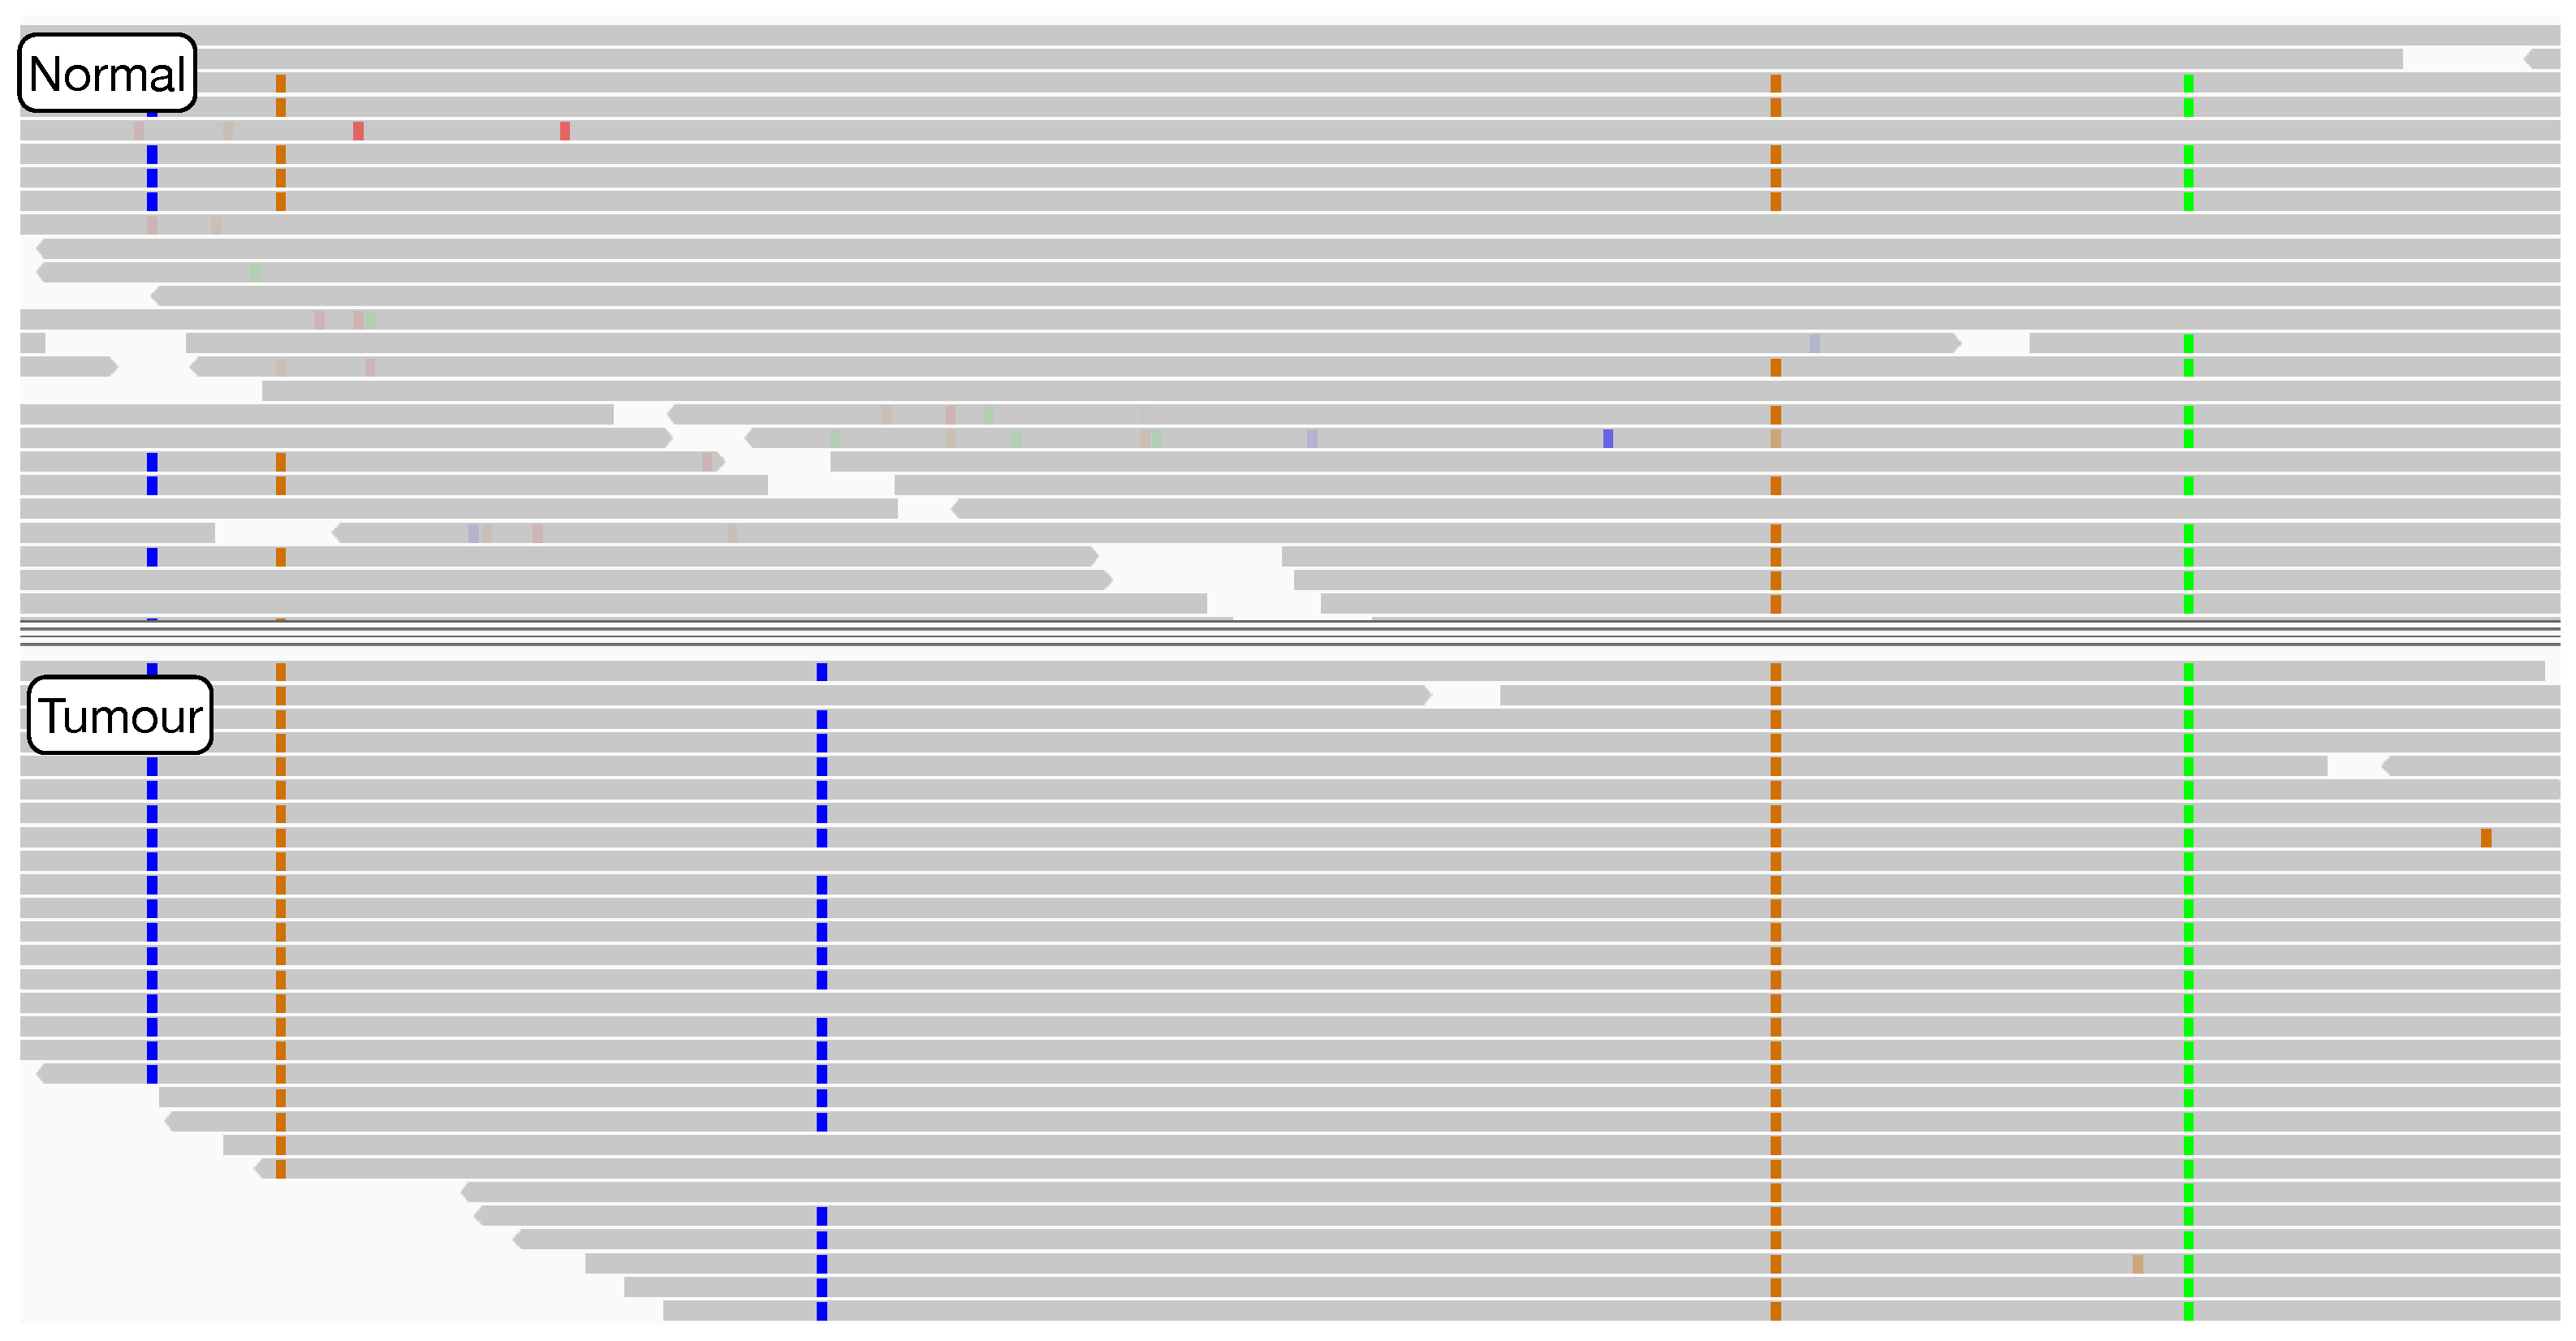
\includegraphics[width=\linewidth]{images/spike_in2}
\end{center}

\end{frame}

\begin{frame}
\frametitle{Phased somatic mutation calls}

\begin{center}
    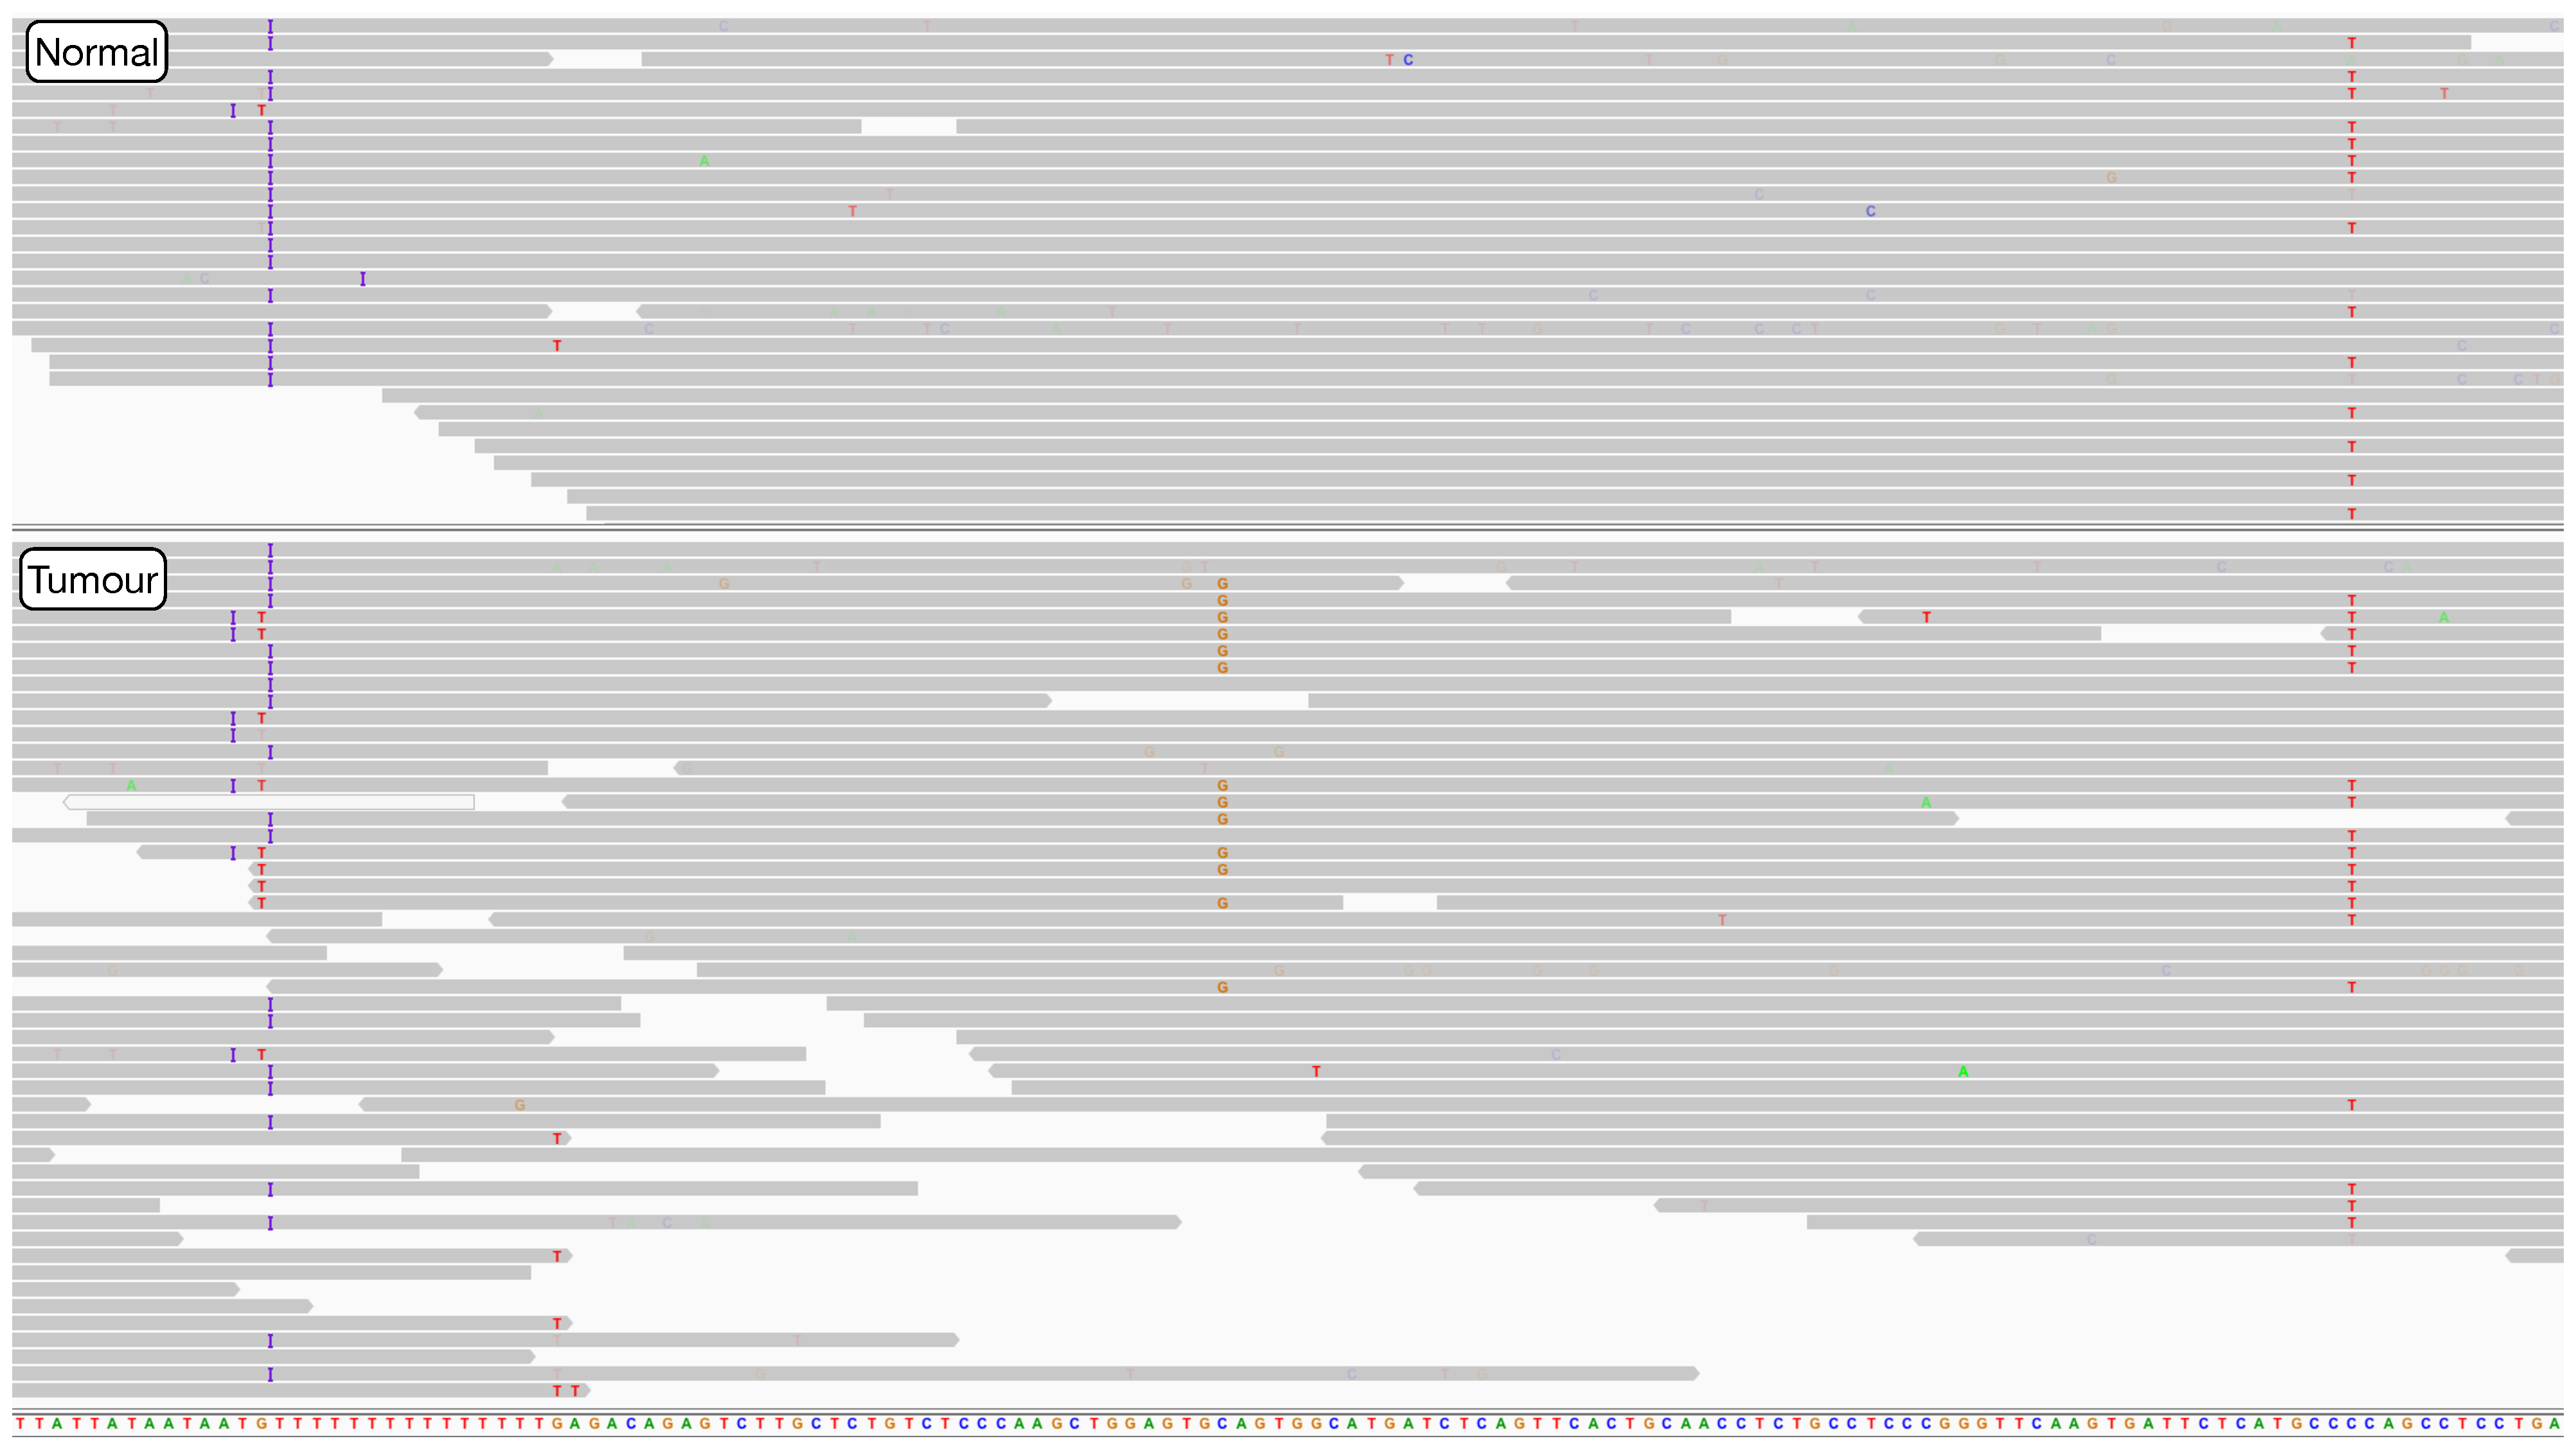
\includegraphics[width=\linewidth]{images/spike_in}
\end{center}

\end{frame}

%------------------------------------------------
\section{Conclusion}
%------------------------------------------------

\begin{frame}
\frametitle{Summary \& future work}
\begin{center}
    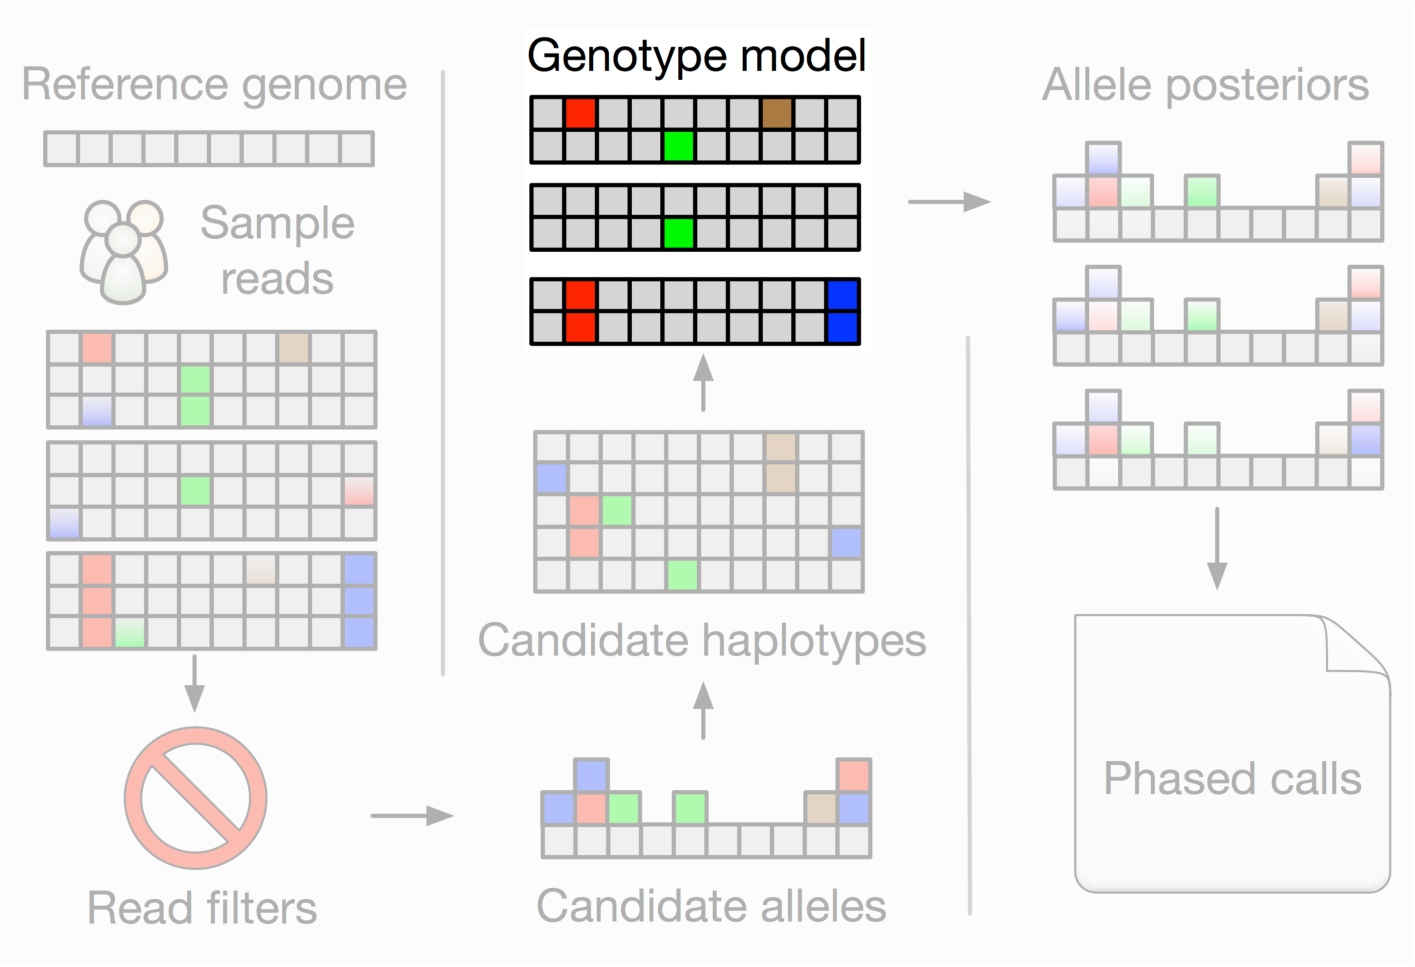
\includegraphics[width=0.95\linewidth]{images/octopus_future}
\end{center}
\end{frame}

%------------------------------------------------

\begin{frame}
\frametitle{Acknowledgements}

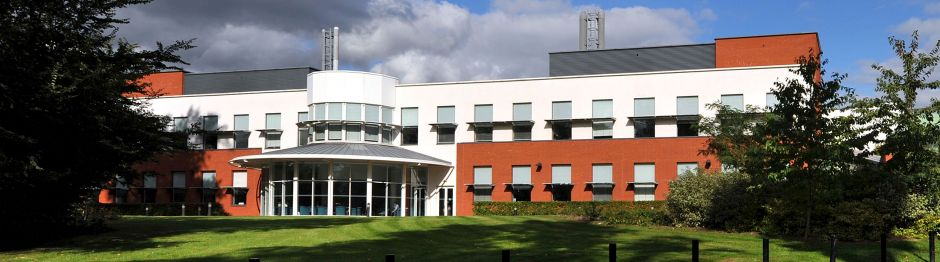
\includegraphics[width=\linewidth]{images/wtchg}

\begin{center}
    
\includegraphics[width=0.2\linewidth]{images/wtchg_logo}
    \hspace{1cm}
    
\includegraphics[width=0.1\linewidth]{images/oxford_logo}
\end{center}

\centerline{Lunter group}
\centerline{with special thanks to Gerton Lunter}
\end{frame}

%----------------------------------------------------------------------------------------

\end{document} 